\documentclass[11pt]{charter}
\usepackage{pdflscape}
\usepackage{hyperref}
\usepackage{ltablex} 
\usepackage{tabularx}
\usepackage{makecell}
%\usepackage{array}
%\newcolumntype{Y}{>{\centering\arraybackslash}X}
%\usepackage{array}

% El títulos de la memoria, se usa en la carátula y se puede usar el cualquier lugar del documento con el comando \ttitle
\titulo{Sistema de control de granja } 

% Nombre del posgrado, se usa en la carátula y se puede usar el cualquier lugar del documento con el comando \degreename
%\posgrado{Carrera de Especialización en Sistemas Embebidos}
\posgrado{Carrera de Especialización en Internet de las Cosas} 
%\posgrado{Carrera de Especialización en Intelegencia Artificial}
%\posgrado{Maestría en Sistemas Embebidos} 
%\posgrado{Maestría en Internet de las cosas}

% Tu nombre, se puede usar el cualquier lugar del documento con el comando \authorname
\autor{Katherine Aguirre} 

% El nombre del director y co-director, se puede usar el cualquier lugar del documento con el comando \supname y \cosupname y \pertesupname y \pertecosupname
\director{William Mercado}
\pertenenciaDirector{UNEG} 
% FIXME:NO IMPLEMENTADO EL CODIRECTOR ni su pertenencia
%\codirector{} % si queda vacio no se deberíá incluir 
%\pertenenciaCoDirector{}

% Nombre del cliente, quien va a aprobar los resultados del proyecto, se puede usar con el comando \clientename y \empclientename
\cliente{Gastón Algaze}
\empresaCliente{Kin and Carta}

% Nombre y pertenencia de los jurados, se pueden usar el cualquier lugar del documento con el comando \jurunoname, \jurdosname y \jurtresname y \perteunoname, \pertedosname y \pertetresname.
\juradoUno{Nombre y Apellido (1)}
\pertenenciaJurUno{pertenencia (1)} 
\juradoDos{Nombre y Apellido (2)}
\pertenenciaJurDos{pertenencia (2)}
\juradoTres{Nombre y Apellido (3)}
\pertenenciaJurTres{pertenencia (3)}
 
\fechaINICIO{22 de junio de 2020}		%Fecha de inicio de la cursada de GdP \fechaInicioName
\fechaFINALPlanificacion{22 de Agosto de 2021} 	%Fecha de final de cursada de GdP
\fechaFINALTrabajo{22 de diciembre de 2021}		%Fecha de defensa pública del trabajo final


\begin{document}

\maketitle
\thispagestyle{empty}
\pagebreak


%-------------------------------------------------------
\section{Registros de cambios}
\label{sec:registro}


\begin{table}[ht]
\label{tab:registro}
\centering
\begin{tabularx}{\linewidth}{@{}|c|X|c|@{}}
\hline
\rowcolor[HTML]{418ddc} 
1.0      & Creación del documento                                          & 26/08/2020 \\ \hline
1.1      & Actualización de los primeros 6 temas                           & 04/09/2020 \\ \hline
1.2      & Incorporación de historias de usuarios                          & 14/09/2020 \\ \hline
1.3      & Correcciones sugeridas y desarrollo hasta el punto 11           & 21/09/2020 \\ \hline
1.4      & Desarrollo hasta el punto 17                           		   & 28/09/2020 \\ \hline
%1.1      & Actualización de los primeros 6 temas                           & 04/09/2020 \\ \hline
%1.1      & Actualización de los primeros 6 temas                           & 04/09/2020 \\ \hline
%\1.2      & Otro ejemplo \newline
%\		   Con texto partido \newline
%\		   En varias líneas \newline
%\		   A propósito                                                     & dd/mm/aaaa \\ \hline \hline
\end{tabularx}
\end{table}

\pagebreak


%-------------------------------------------------------
\section{Acta de constitución del proyecto}
\label{sec:acta}

\begin{flushright}
Buenos Aires, \fechaInicioName
\end{flushright}

\vspace{2cm}

Por medio de la presente se acuerda con la Ing. \authorname\hspace{1px} que su Trabajo Final de la \degreename\hspace{1px} se titulará ``\ttitle'', consistirá esencialmente en el diseño de un Sistema de Monitoreo y Control de Variables Medioambientales en una Granja, y tendrá un presupuesto preliminar estimado de 600 hs de trabajo  y 299.844,77 ARP, con fecha de inicio \fechaInicioName\hspace{1px} y fecha de presentación pública \fechaFinalName.

Se adjunta a esta acta la planificación inicial.

\vfill

% Esta parte se construye sola con la información que hayan cargado en el preámbulo del documento y no debe modificarla
\begin{table}[ht]
\centering
\begin{tabular}{ccc}
\begin{tabular}[c]{@{}c@{}}Ariel Lutenberg \\ Director posgrado FIUBA\end{tabular} & \hspace{2cm} & \begin{tabular}[c]{@{}c@{}}\clientename \\ \empclientename \end{tabular} \vspace{2.5cm} \\ 
\multicolumn{3}{c}{\begin{tabular}[c]{@{}c@{}} \supname \\ Director del Trabajo Final\end{tabular}} \vspace{2.5cm} \\
%\begin{tabular}[c]{@{}c@{}}\jurunoname \\ Jurado del Trabajo Final\end{tabular}     &  & \begin{tabular}[c]{@{}c@{}}\jurdosname\\ Jurado del Trabajo Final\end{tabular}  \vspace{2.5cm}  \\
%\multicolumn{3}{c}{\begin{tabular}[c]{@{}c@{}} \jurtresname\\ Jurado del Trabajo Final\end{tabular}} \vspace{.5cm}                                                                     
\end{tabular}
\end{table}


%-------------------------------------------------------
\section{Descripción técnica-conceptual del proyecto a realizar}
\label{sec:descripcion}

\begin{consigna}{black} 
Referenciando al prototipo conceptual del Sistema de Control Granja se crea la necesidad de diseñar y desarrollar un sistema acorde a los requerimientos actuales de tecnología, comunicaciones y seguridad que se adecuen al criterio de Internet de las Cosas manejado hoy día, de esta manera se origina un proyecto basado en la premisa de automatizar tareas de monitoreo continuo de temperatura, humedad, calidad del aire, flujo de agua y activación de sistemas de acondicionamiento ambiental de las naves de las granjas de producción animal bajo condiciones controladas, garantizando así el poder adecuarlas a los valores de bienestar ideal que optimizan la crianza de animales y productos relacionados para el consumo humano. 

El planteamiento parte del \textit{knowhow} obtenido en el desarrollo del prototipo conceptual del Sistema de Control Granja, entendiendo el ¿por qué? de las fallas encontradas tanto de seguridad como de latencia, comunicaciones, diseño entre otros, aplicando las buenas practicas que rigen para el desarrollo de este tipo de soluciones y generar de esta manera un producto robusto que reduzca al mínimo probable dichas falencias y converja al máximo posible entre la eficiencia y la eficacia.

Del mismo modo, en la Figura \ref{fig:diagBloques} se puede observar el diagrama de bloques que conformará el nuevo sistema, el cual contara con los siguientes módulos: 
\begin{enumerate}
\item Sensores y Actuadores: conjunto de dispositivos cuya finalidad es la de capturar la telemetría o ejecutar ciertas acciones. Contarán con un portal cautivo.
\begin{itemize}
\item Portal Cautivo: sistema de administración de los sensores.
\end{itemize}
\item Broker MQTT: servicio que se encargará de recepcionar los mensajes enviados por los clientes y distribuirlos entre sí en el sistema pub-sub (publicación - suscripción de tópicos).
\item Servicio NTP: Permitirá sincronizar los relojes de los sensores con el servidor.
\item Api - WebService: servicio que permitirá el intercambio de datos entre las aplicaciones.
\item Motor de Base de Datos: repositorio para almacenamiento y persistencia de los datos.
\item Aplicaciones: software para interactuar con los distintos bloques que integran el sistema, a saber:
	\begin{itemize}
		\item App Web: sistema alojado en el servidor que podrá ser accedido vía wrobser.
		\item App Mobile: sistema para dispositivos móviles.
		\item Sistema de Mensajería y Alertas: Sistema de soporte para el manejo de eventualidades, reportes o alertas.
	\end{itemize}
\end{enumerate}

\vspace{25px}

\begin{figure}[htpb]
\centering 
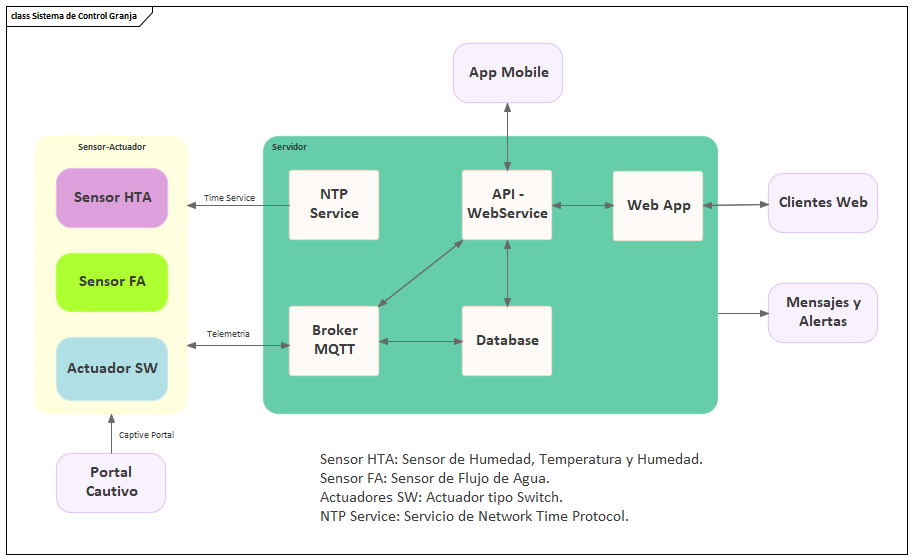
\includegraphics[width=1\textwidth]{./Figuras/diagBloques.png}
\caption{Diagrama en bloques del sistema}
\label{fig:diagBloques}
\end{figure}

\vspace{25px}
\end{consigna}


%-------------------------------------------------------
\section{Identificación y análisis de los interesados}
\label{sec:interesados}

\begin{consigna}{black} 
%Nota: (borrar esto y todas las consignas en color rojo antes de entregar este documento).
% 
%Es inusual que una misma persona esté en más de un rol, incluso en proyectos chicos.
% 
%Si se considera que una persona cumple dos o más roles, entonces sólo dejarla en el rol más importante. Por ejemplo:
%
%\begin{itemize}
%\item Si una persona es Cliente pero también colabora u orienta, dejarla solo como Cliente.
%\item Si una persona es el Responsable, no debe ser colocado también como Miembro del equipo.
%\end{itemize}
%
%Pero en cambio sí es usual que el Cliente y el Auspiciante sean el mismo, por ejemplo.


\begin{table}[ht]
%\caption{Identificación de los interesados}
%\label{tab:interesados}
\begin{tabularx}{\linewidth}{@{}|l|X|X|l|@{}}
\hline
\rowcolor[HTML]{418ddc} 
Rol           & Nombre y Apellido & Organización 	& Puesto 	\\ \hline
%Auspiciante   & -                 & -           	& -     	\\ \hline
Cliente       & Gastón Algaze                 & Kin and Carta           	& Managing Director   	\\ \hline
%Impulsor      & -                 & -            	& -      	\\ \hline
Responsable   & \authorname       & FIUBA        	& Alumno 	\\ \hline
Colaboradores & Gisvel Gonzalez                & Freelancer            	& UX/UI Designer      	\\ \hline
Orientador    & \supname	      & \pertesupname 	& Director	Trabajo final \\ \hline
%Equipo        & - & -	& -   	\\ \hline
%Opositores    & -                 & -            	& -      	\\ \hline
%Usuario final & -                 & -            	& -      	\\ \hline
\end{tabularx}
\end{table}

%El Director suele ser uno de los Orientadores.
%
%No dejar celdas vacías; si no hay nada que poner en una celda colocar un signo ``-''.
%
%No dejar filas vacías; si no hay nada que poner en una fila entonces eliminarla.
%
%Sería deseable listar a continuación de la tabla las principales características de cada interesado.
% 
%Por ejemplo:
%\begin{itemize}
%\item Auspiciante: es riguroso y exigente con la rendición de gastos. Tener mucho cuidado con esto.
%\item Equipo: Juan Perez, suele pedir licencia porque tiene un familiar con una enfermedad. Planificar considerando esto.
%\item Orientador: María Gómez, nos va a poder ayudar mucho con la gestión de impuestos.
%\end{itemize}

\end{consigna}


%-------------------------------------------------------
\hfill \break
\section{1. Propósito del proyecto}
\label{sec:proposito}
\begin{consigna}{black} 
El propósito de este proyecto es el de diseñar y producir un Sistema para Monitoreo y Control de Variables Medioambientales enfocado a granjas de producción animal, aplicando las buenas practicas que rigen en el desarrollo de soluciones IoT de manera óptima, tomando como referencia un prototipo conceptual basado en granja avícola.
\end{consigna}


%-------------------------------------------------------
\newpage
\section{2. Alcance del proyecto}
\label{sec:alcance}

\begin{consigna}{black}
%¿Qué se incluye y que no se incluye en este proyecto?
%
%Se refiere al trabajo a hacer para entregar el producto o resultado especificado. 
%
%Explicitar todo lo quede comprendido dentro del alcance del proyecto.
%
%Explicitar además todo lo que no quede incluido (``El presente proyecto no incluye...'')
El alcance del proyecto contempla el desarrollo e implementación de los distintos módulos que componen el sistema en su totalidad y las tareas complemantarias que ayudaran a alcanzar los objetivos planteados, a saber:

\begin{enumerate}
	\item \textbf{Realizar capacitaciones y entrenamientos necesarios para completar los desarrollos en las teconologías seleccionadas}: es mandatorio realizar capacitaciones en diversas teconologías de desarrollo de software para poder completar las tareas, se requiere entrenamiento en: GraphQL y React Native.
	\item \textbf{Configuración del servidor}: se contempla la instalación y configuración de Raspbian Buster lite para plataforma X86 en una Raspberry Pi, así como la generación de certificados para la configuración de las conexiones seguras.	
	\item \textbf{Diseño e implementación de la Base de Datos}: se debe definir el esquema y diagramas de la base datos, así como también realizar la codificación y construcción de la misma en el motor de base de datos seleccionado.
	\item \textbf{Implementación del servicio NTP}: se deben realizar las instalaciones y configuraciones necesarias para poner en funcionamiento el servicio de \textit{Network Time Protocol}.
	\item \textbf{Implementación del Broker MQTT}: se necesita instalar, configurar y securizar el servidor MQTT así como configurar la conexión con la base de datos para persistir la telemetria.
	\item \textbf{Diseño, desarrollo e instalación del software en los sensores}: se necesita desarrollar el sistema de administración de los sensores así como la implementación de los protocolos de comunicación y seguridad necesarios para el envío y recepción de telemetría.
	\item \textbf{Diseño, desarrollo e implementación de la API-WebService}: se debe desarrollar e implementar el WebService que permitirá interactuar a los diferentes clientes con el resto de los módulos habilitados para ello.
	\item \textbf{Diseño, desarrollo e implementación de la App Hibrida}: desarrollar e instalar, según la tecnología, las aplicaciones web y móviles que interactuarán con el WebService.
	\item \textbf{Pruebas Generales del sistema}: cada uno de los módulos que compone el sistema deberá ser testeado para asegurar la calidad y funcionamiento de los mismos.
	\item \textbf{Elaboración de los manuales de configuración e instalación de cada modulo}: es mandatorio elaborar los manuales de instalación, configuración y/o uso de cada modulo desarrollado.
\end{enumerate}
\end{consigna}


%-------------------------------------------------------
\section{3. Supuestos del proyecto}
\label{sec:supuestos}

\begin{consigna}{black}
Para el desarrollo del presente proyecto se supone que: 

\begin{itemize}
	\item El hardware de los sensores y actuadores ya está elaborado por lo que el desarrollo de los mismos se limita al desarrollo e instalación del software, igualmente se cuenta con el hardware y software necesario para configurar el servidor y las estaciones de desarrollo donde será construido  el proyecto.
	\item Se determinó satisfactoriamente la factibilidad técnica del desarrollo de los distintos elementos que componen el proyecto.
	\item Se determinó que existe la disponibilidad de tiempo para recibir capacitación, diseñar, desarrollar e implementar todo el proyecto.
	\item Respecto a las reglamentaciones y leyes existentes se determinó que no existe impedimento alguno para culminar exitosamente el proyecto.
	\item Respecto a la situación presupuestaria del equipo de desarrollo se determinó que no existe impedimento alguno para subsanar los gastos e inversiones necesarias para completar el proyecto.
\end{itemize}
%
%Por ejemplo, se podrían incluir supuestos respecto a disponibilidad de tiempo y recursos humanos y materiales, sobre la factibilidad técnica de distintos aspectos del proyecto, sobre otras cuestiones que sean necesarias para el éxito del proyecto como condiciones macroeconómicas o reglamentarias.
\end{consigna}


%-------------------------------------------------------
\section{4. Requerimientos}
\label{sec:requerimientos}

\begin{consigna}{black}
Los requerimientos necesarios para el desarrollo del proyecto son los siguientes:
\begin{enumerate}
\item Grupo de requerimientos asociados con sensores y actuadores:
	\begin{enumerate}
		\item Deberá activarse en modo servidor cuando no esté conectado a una SSID externa y de esta manera activar el portal de configuración del mismo en un servidor local, una vez conectado a la WiFi externa se deshabilitará la WiFi interna (ésta sólo estará activa en casos de desconexión con la WiFi externa) y funcionará como servidor web donde podrá ser consultada su funcionalidad y telemetría.
		\item Dentro de los servicios a manejar o configurar en el dispositivo se tienen: MQTT (suscripción y publicación de tópicos), NTP, acceso a la telemetría, administración de redes WiFi tanto interna como externa, administración de usuario y contraseña, reset valores de fábrica, reinicio del dispositivo, test de hardware.
		\item Se contempla la actualización remota de los dispositivos habilitando la opción update OTA en los mismos.
		\item Se requiere que las comunicaciones se realicen en formato JSON.
		\item Deberá ser capaz de publicar datos de su funcionamiento para que sean registrados y procesados posteriormente según sea la necesidad, estas comunicaciones deberán estar encriptadas mediante el uso de comunicaciones seguras con SSL/TLS, usuario y contraseña para garantizar la privacidad en el transporte de datos.
		\item Deberá poder conectarse a un servidor NTP para tener su hora sincronizada y así poder manejar cabeceras de tiempo en los registros enviados en formato JSON.
	\end{enumerate}
\item Grupo de requerimientos asociados con el servicio NTP:
	\begin{enumerate}
		\item Se deberá contar con un servicio de hora que pueda funcionar \emph{offline} en caso de fallar la conectividad a internet para así poder sincronizar las operaciones.
	\end{enumerate}
\item Grupo de requerimientos asociados con la base de datos:
	\begin{enumerate}
		\item Se requiere la instalación y configuración del motor de base de datos para su posterior uso, el cual deberá ser Postgres o MongoDB en su defecto.\newpage
		\item Se requiere diseñar y elaborar el esquema de la base de datos según los siguientes puntos:
			\begin{enumerate}
				\item Usuarios
				\item Roles
				\item Alarmas, mensajes y escalas de severidades.
				\item Permisos
				\item Estados
				\item Zonas de acción
				\item Lecturas de datos
				\item Telemetría
				\item Dispositivos
				\item Tipos bases
			\end{enumerate}
		\item Se requiere que los datos puedan ser registrados en formato JSON.
	\end{enumerate}
\item Grupo de requerimientos asociados con el broker MQTT:
	\begin{enumerate}
		\item Se requiere la instalación y configuración de Mosquitto como gestor de Pub-Sub.
		\item Publicación: telemetría, estatus del dispositivo, potencia de la señal wifi, versión del firmware.
		\item Suscripción: activación o desactivación de actuadores de forma manual según el tiempo definido, requerir datos específicos por ítem de los mencionados en el punto previo.
		\item Registro de datos en la Base de Datos.
		\item Se requiere que las comunicaciones se realicen en formato JSON.
	\end{enumerate}	
\item Grupo de requerimientos asociados con Api - WebService:
	\begin{enumerate}
		\item En un principio se plantea la posibilidad de desarrollar la Api en GraphQL con Node.js, sino es factible se empleará Spring Boot 2 sobre Apache Tomcat.
		\item Deberá manejar inicios de sesión autenticados así como comunicaciones seguras tanto con el Broker como con los clientes y la base de datos.
		\item Se contempla que la API sea capaz de enviar alertas de alarmas vía email, tweets, chats de telegram o mensajes IFTTT.
		\item Se requiere que las comunicaciones se realicen en formato JSON.
		\item Dentro de los endpoints a definir se encuentran los siguientes gestiones:
		\begin{itemize}
		\item Usuarios.
		\item Roles de usuarios.
		\item Configuraciones varias
		\item Tipos: alarmas, sensores
		\item Zonas a monitorear.
		\item Permisos.
		\item Estados.
		\item Sensores.
		\item Lecturas de Datos
		\item Alarmas generadas
		\item Escala de severidades de alarmas
		\item Categorías de clasificación de registros
		\item Consulta de telemetría por sensor.
		\item Activación de actuadores.
		\item MQTT: suscripción y publicación de tópicos
		\item NTP
		\end{itemize}
	\end{enumerate}	
\item Grupo de requerimientos asociados con la App:
	\begin{enumerate}
		\item El cliente será una App basada en JS, se plantea la posibilidad de hacerla multiplataforma con soporte para dispositivos mobile (Android, IOS) y para navegadores (Chrome, Firefox, Safari) tanto de escritorios (Windows, MacOS, Linux) como tablets (Android, Ipad). 
		\item Se requiere SSL/TLS en todas las comunicaciones.
		\item Se recomienda el uso de React Native.
		\item Se requiere que las comunicaciones se realicen en formato JSON.
	\end{enumerate}		
\end{enumerate}
%
%Leyendo los requerimientos se debe poder interpretar cómo será el proyecto y su funciónalidad.
%
%De ser posible indicar cómo se obtuvieron cada uno de los requerimientos 
%
%Indicar claramente cuál es la prioridad entre los distintos requerimientos. 
%
%No olvidarse de que los requerimientos incluyen a las regulaciones y normas vigentes!!!
%
%Y al escribirlos seguir las siguientes reglas:
%\begin{itemize}
%\item Ser breve y conciso (nadie lee cosas largas). 
%\item Ser específico: no dejar lugar a confusiones.
%\item Expresar los requerimientos en términos que sean cuantificables y medibles.
%\end{itemize}
\end{consigna}


%-----------------------------------------------------------
\begin{landscape}

\section{Historias de usuarios (\textit{Product backlog})}
\label{sec:backlog}
\vspace*{1px}
Las historias de usuarios se encuentran diseñadas para emplear SCRUM como metodología de trabajo: 

\begin{tabularx}{\linewidth}{@{}|p{1.3cm}|p{17cm}|p{1.7cm}|p{1.5cm}|p{1.7cm}|@{}}
      \hline 
      \rowcolor[HTML]{C0C0C0} 
      \textbf{Clave} & \textbf{Resumen} & \textbf{Prioridad} & \textbf{Points} & \textbf{Estimado}\\ \hline
PG-1     & Realizar entrenamiento en   GraphQL  & Highest            & 13  & 14,0  Hrs         \\
         &  \begin{description}        
                   \item Como Product Owner requiero que los miembros del equipo de desarrollo se capaciten en GraphQL entonces podrán desarrollar la API sin inconvenientes.            
                   \textbf{Detalles Técnicos:} \href{https://www.udemy.com/course/graphql-with-react-course/}{graphql-with-react-course}         
                    \item Testing:
            \end{description}  &  &     & \\
            
PG-2     & Realizar entrenamiento en React   Native         & High               & 20  & 20,0  Hrs         \\
         &  \begin{description}
                   \item Descripción:  Como Product Owner quiero que los miembros del equipo de desarrollo se capaciten en React Native entonces podrán trabajar en el desarrollo de las aplicaciones híbridas sin inconvenientes.                 
                   \item Testing:
            \end{description}            &  &     & \\            
PG-11    & Bases de datos: Instalación,   configuración y testeo.             & High               & 5   & 22,0  Hrs         \\
         &  \begin{description}          
                   \item Descripción:  Como Developer, requiero tener la infraestuctura necesaria para que   almacenar los datos de los programas                 
                   \item \textbf{Criterio de Aceptación:} DADO que tanto el Broker como la API necesitan almacenamiento permanente e   intercambio de datos CUANDO tanto los sensores como las aplicaciones clientes lo requieran ENTONCES se necesita instalar y configurar un motor de base de datos relacional y uno no relacional,  Y a su vez se debe popular el esquema de la base de datos según el documento anexo.
                   \item \textbf{Scope:} Se debe tener el servidor previamente configurado      
				   \textbf{Detalles Técnicos:}
                   \begin{description} 
                         \item la base de datos a instalar es Postgresql 12 y MongoDB 
                         \item se debe configurar la BD para que acepte conexiones externas 
                         \item se requiere habilitar SSL siempre que sea técnicamente posible 
                         \item emplear el .backup anexo para popular la DB 
				   \end{description}
                   \item Testing:
            \end{description}    &  &     & \\ 
PG-32    & Configurar el Servidor         & High               & 13  & 14,0  Hrs         \\
         &  \begin{description}
				   \item Como administrador, quiero   contar con el servidor configurado para que se puedan deployar los   desarrollos.                 
                   \item \textbf{Criterio de Aceptación:}
				   \begin{description} 
					\item DADO que inicialmente el servidor no cuenta con OS alguno CUANDO el hardware se encuentra nuevo ENTONCES se  instalar el OS                 				
					\item DADO que se requiere configurar el OS CUANDO ya se encuentre instalado  ENTONCES se procederá a ejecutar su configuración
					\item DADO que se deberán securizar las comunicaciones con TLS/SSL CUANDO se desarrolle el proyecto ENTONCES se requerirá generar los certificados correspondientes
					\item DADA cualquier labor de mantenimiento del servidor CUANDO se requiera realizar alguna acción mediante una interfaz amigable   sin recurrir a la consola ENTONCES se procederá a instalar WebMin 
					\item DADO que se requiere un software para almacenar contenedores CUANDO se requiera consumir algún recurso del servidor  ENTONCES se procederá a instalar Docker Y \href{http://Portainer.io}{Portainer.io} como administrador de   contenedores.                 
					\item DADO que se requiere un broker MQTT CUANDO se requiera de comunicación bidireccional con los sensores y   actuadores ENTONCES se procederá a instalar Mosquitto Y se procederá a configurarlo según requerimientos                 
					\item DADO que se requiere un servicio NTP CUANDO se requiera cronometrar las comunicaciones por MQTT ENTONCES se procederá a configurar un contenedor con un servidor NTP Y se procederá a configurarlo                 
					\item DADO que se requiere un manual con todos los procedimientos de configuración CUANDO ENTONCES se procederá documentar todo el proceso 
				\end{description}
				\item \textbf{Fuera de Alcance:}	     
					\begin{description} 
                         \item OS a instalar: Raspbian lite 
                         \item Seguir guía de instalación y configuración adjunta 			   
                         \item Administrador web para el server: WebMin 			   
                         \item Administrador de contenedores: Docker + portainer 				
                         \item Servicio de hora: contenedor NTP					   			   
                         \item Broker de comunicaciones: Mosquitto MQTT  
					\end{description}
                   \item Testing:
            \end{description} &  &     & \\
PG-99    & Backend: Creación de la   documentación - Instalación y Configuración.               & Medium             & 13  & 36,0  Hrs         \\
         &  \begin{description}
                   \item Como administrador, quiero   contar con documentación técnica detallada relacionada con las capabilities   que ofrece el Backend del sistema así poder consultar la información cuando   
				 así lo requiera o poderla compartir con el equipo de desarrollo ante cualquier   consulta.                 
                   \item \textbf{Criterio de Aceptación:}
                   \item DADO que se requiere contar con la documentación del backend CUANDO       ENTONCES se procede a realizar la documentación detallada de los endpoints   del Backend.                
                   \item \textbf{Scope:}
                         \item Se requiere: detallar lo máximo posible cada endpoint a fin de facilitar   la posterior consulta de los mismos 
                         \item Se sugiere la creación de un swagger                 
                   \item Testing: No aplica
            \end{description}            &  &     & \\
PG-170   & Frontend: Creación de la   documentación - Instalación y Configuración.              & Medium             & 13  & 36,0  Hrs         \\
         &  \begin{description}
                   \item Como administrador, quiero   contar con documentación técnica detallada relacionada con las capabilities   que ofrece el Frontend del sistema así poder consultar la información cuando   así lo requiera o poderla compartir con el equipo de desarrollo ante cualquier   duda generada.                 
                   \item \textbf{Criterio de Aceptación:}
                   \item DADO que se requiere contar con la documentación del frontend CUANDO       ENTONCES se procede a realizar la documentación detallada de las   funcionalidades del Frontend.                
                   \item \textbf{Scope:}
                         \item Se requiere: detallar lo máximo posible cada funcionalidad a fin de   facilitar la posterior consulta de los mismos                 
                   \item Testing: No aplica
            \end{description}  &  &     & \\
PG-197   & Portal Cautivo: Documentación y   creación del Manual de configuración               & Medium             & 3   & 32,0  Hrs         \\
         &  \begin{description}
                   \item Como administrador, quiero tener   la documentación del portal cautivo y así poder tenerla de referencia para   futuras consultas                 
                   \item \textbf{Criterio de Aceptación:}
                   \item DADO que se requiere poder tener el manual de configuración del portal cautivo CUANDO se requiera realizar alguna acción en el sensor desde el ámbito   administrativo ENTONCES se procede a desarrollar la funcionalidad necesaria para poder   suplir dicho requerimiento en Arduino / C++                
                   \item Testing:
            \end{description}   &  &     & \\
PG-44    & Backend: Desarrollar endpoints   para gestión de sesiones seguras  & Medium             & 13  & 17,4  Hrs         \\
         &  \begin{description}                 
                   \item Como usuario, requiero poder   hacer inicio o cierre de sesiones seguras en mis aplicaciones (mobile y Web)   para que pueda empezar a interactuar con el sistema.                 
                   \item \textbf{Criterio de Aceptación:}                 
                   \item DADO que se requiere poder hacer inicios de sesión seguros en las   aplicaciones (mobile y Web) CUANDO las aplicaciones soliciten los recursos necesarios para realizar   tales acciones ENTONTES se procede a desarrollar las Endpoints para inicio y cierre de   sesión                 
                         \item El equipo de desarrollo debe configurar las herramientas y tener el   entorno de desarrollo habilitado                 
                   \item Testing:                 
            \end{description}            &  &     & \\
PG-47    & Frontend: Desarrollar inicio de   sesiones seguras en la App mobile y Web            & Medium             & 21  & 27,4  Hrs         \\
         &  \begin{description}                 
                   \item Como usuario, requiero poder   hacer inicio o cierre de sesiones seguras en mis aplicaciones (mobile y Web)   para que pueda empezar a interactuar con el sistema.                 
                   \item \textbf{Criterio de Aceptación:}                 
                   \item DADO que se requiere poder hacer inicios de sesión seguros en las   aplicaciones (mobile y Web) CUANDO el usuario así lo requiera ENTONCES se procede a desarrollar las funcionalidades: Iniciar sesión,   Cierre de Sesión
					\item El equipo de desarrollo debe configurar las herramientas y tener el   entorno de desarrollo habilitado                 
                   \item Testing:                 
                   \item \textbf{Scope:}
            \end{description}   &  &     & \\
PG-51    & Backend: Desarrollar endpoints   GraphQL para gestión del espacio del usuario        & Medium             & 8   & 7,4  Hrs          \\
         &  \begin{description}                 
                   \item Como usuario, quiero poder   gestionar la información contenida en mi espacio para que pueda tener mis   datos actualizados en las aplicaciones.                 
                   \item \textbf{Criterio de Aceptación:}                 
                   \item DADO que se requiere poder hacer modificación de datos en los espacios de   los usuarios para las aplicaciones (mobile y Web) CUANDO las aplicaciones soliciten los recursos necesarios para realizar   tales acciones ENTONCES se procede a desarrollar las Endpoints para gestión de datos del   usuario
                   \item Testing:                 
            \end{description}          &  &     & \\   
PG-52    & Frontend: Crear la gestión del   espacio de usuario en las aplicaciones.             & Medium             & 8   & 13,4  Hrs         \\
         &  \begin{description}                 
                   \item Como usuario, quiero poder   gestionar la información contenida en mi espacio para que pueda tener mis   datos actualizados en las aplicaciones.                 
                   \item \textbf{Criterio de Aceptación:}                 
                   \item DADO que se requiere poder hacer modificación de datos en los espacios de   los usuarios para las aplicaciones (mobile y Web) CUANDO las aplicaciones soliciten los recursos necesarios para realizar   tales acciones ENTONCES se procede a desarrollar las pantallas necesarias para gestion de   datos del usuario                          
                   \item Testing:                 
            \end{description}                 &  &     & \\
PG-74    & Backend: Creación del endpoint   para la suscripción y publicación de tópicos.       & Medium             & 3   & 13,4  Hrs         \\
         &  \begin{description}                 
                   \item Como usuario, quiero poder   interactuar con los sensores a través de la telemetría para poder realizar   consultas de estados o datos.                 
                   \item \textbf{Criterio de Aceptación:}                 
                   \item DADO que se requiere poder tener comunicación con los sensores mediante el   Broker MQTT CUANDO se requiera revisar el estado de los sensores, consultar algún dato   o ejecutar una acción ENTONCES se procede a desarrollar el endpoint necesario para poder suplir dicho requerimiento en GraphQL                
                   \item \textbf{Scope:}                  
                         \item Se requiere: Consultar, editar o inhabilitar registros, 
                         \item No se permite eliminar registros 
                         \item Cada registro es dependiente del tiempo                 
                   \item Testing:
            \end{description}        &  &     & \\
PG-80    & Backend: Creación del endpoint   para la Gestión de Alarmas y Notificaciones         & Medium             & 3   & 7,4  Hrs          \\
         &  \begin{description}                 
                   \item Como administrador, quiero poder   las Alarmas o Alertas generadas por el sistema y así poder realizar las   tareas administrativas necesarias.                 
                   \item \textbf{Criterio de Aceptación:}                 
                   \item DADO que se requiere poder gestionar las Alarmas y Alertas del   sistema CUANDO se requiera realizar alguna acción sobre los registros desde el   ámbito administrativo ENTONCES se procede a desarrollar el endpoint necesario para poder suplir dicho requerimiento en GraphQL                
                   \item \textbf{Scope:}                  
                         \item Se requiere: Consultar, editar o inhabilitar registros, 
                         \item No se permite eliminar registros 
                         \item Cada registro es dependiente del tiempo                 
                   \item Testing:
            \end{description}  &  &     & \\
PG-95    & Backend: Creación del endpoint   para la Lectura de Datos generados.                 & Medium             & 13  & 38,8  Hrs         \\
         &  \begin{description}                 
                   \item Como usuario, quiero consultar   los datos por los sensores tanto por dispositivo como por zona y así poder   monitorear el estado de las variables ambientales.                 
                   \item \textbf{Criterio de Aceptación:}                 
                   \item DADO que se requiere poder consultar los datos generados por los   sensores CUANDO se requiera realizar alguna acción sobre los registros de   lecturas ENTONCES se procede a desarrollar el endpoint necesario para poder suplir dicho requerimiento en GraphQL                
                   \item \textbf{Scope:}             
                         \item Se requiere: Consultar registros, 
                         \item No se permite eliminar o editar registros 
                         \item Se requiere que las queries puedan consultar uno (01) o mas sensores /   zonas a la vez, así como periodo de tiempo en minutos, horas, días y   semanas                 
                   \item Testing:
            \end{description}          &  &     & \\                     
PG-138   & Frontend: Creación de la   funcionalidad para la Gestión de Alarmas y Notificaciones.& Medium             & 5   & 7,4  Hrs          \\
         &  \begin{description}                 
                   \item Como administrador, quiero poder   las Alarmas o Alertas generadas por el sistema y así poder realizar las   tareas administrativas necesarias.                 
                   \item \textbf{Criterio de Aceptación:}                 
                   \item DADO que se requiere poder gestionar las Alarmas y Alertas del   sistema CUANDO se requiera realizar alguna acción sobre los registros desde el   ámbito administrativo ENTONCES se procede a desarrollar la funcionalidad necesaria para poder   suplir dicho requerimiento en React Native                
                   \item \textbf{Scope:}                  
                         \item Se requiere: Consultar, editar o inhabilitar registros, 
                         \item No se permite eliminar registros                 
                   \item Testing:
            \end{description}      &  &     & \\
PG-142   & Frontend: Creación de la   funcionalidad para la suscripción y publicación de tópicos.                 & Medium             & 5   & 13,4  Hrs         \\
         &  \begin{description}                 
                   \item Como usuario, quiero poder   interactuar con los sensores a través de la telemetría para poder realizar   consultas de estados o datos.                 
                   \item \textbf{Criterio de Aceptación:}                 
                   \item DADO que se requiere poder tener comunicación con los sensores mediante el   Broker MQTT CUANDO se requiera revisar el estado de los sensores, consultar algún dato   o ejecutar una acción ENTONTES se procede a desarrollar la funcionalidad necesaria para poder   suplir dicho requerimiento en React Native                
                   \item \textbf{Scope:}                  
                         \item Se requiere: Consultar, editar o inhabilitar registros, 
                         \item No se permite eliminar registros                 
                   \item Testing:
            \end{description}            &  &     & \\
PG-166   & Frontend: Creación de la   funcionalidad para la Lectura de Datos generados.         & Medium             & 21  & 38,8  Hrs         \\
         &  \begin{description}                 
                   \item Como usuario, quiero consultar   los datos por los sensores tanto por dispositivo como por zona y así poder   monitorear el estado de las variables ambientales.                 
                   \item \textbf{Criterio de Aceptación:}                 
                   \item DADO que se requiere poder consultar los datos generados por los   sensores CUANDO se requiera realizar alguna acción sobre los registros de   lecturas ENTONCES se procede a desarrollar funcionalidad necesaria para poder suplir dicho requerimiento en React Native                
                   \item \textbf{Scope:}                  
                         \item Se requiere: Consultar registros, 
                         \item No se permite eliminar o editar registros 
                         \item Se requiere que las queries puedan consultar uno (01) o mas sensores /   zonas a la vez, así como periodo de tiempo en minutos, horas, días y   semanas                 
                   \item Testing:
            \end{description}   &  &     & \\
PG-58    & Backend: Creación del endpoint   para la Gestión de Permisos       & Medium             & 3   & 7,4  Hrs          \\
         &  \begin{description}                 
                   \item Como administrador, quiero poder   gestionar los permisos de usuarios para poder realizar correctamente las   gestiones de seguridad del sistema.                 
                   \item \textbf{Criterio de Aceptación:}                 
                   \item DADO que se requiere poder administrar los distintos permisos que pueden   tener los usuarios. CUANDO se estén realizando tareas de administración de usuarios. ENTONCES se procede a desarrollar el endpoint necesario para poder suplir dicho requerimiento en GraphQL             
                   \item Fuera de Alcance:                 
                   \textbf{Detalles Técnicos:} 
                         \item Se requiere: Consultar, editar o inhabilitar registros, 
                         \item No se permite eliminar registros 
                         \item Cada registro es dependiente del tiempo                 
                   \item Testing:                 
            \end{description}        &  &     & \\

PG-62    & Backend: Creación del endpoint   para la Gestión de Estados        & Medium             & 3   & 7,4  Hrs          \\
         &  \begin{description}                 
                   \item Como administrador, quiero poder   gestionar los estados de todos los registros de la base de datos.                 
                   \item \textbf{Criterio de Aceptación:}                 
                   \item DADO que se requiere poder administrar los distintos estados que pueden   tener los registros en la base de datos. CUANDO se estén realizando tareas de administración, creando o actualizando   datos o registros. ENTONCES se procede a desarrollar el endpoint necesario para poder suplir dicho requerimiento en GraphQL                           
                   \textbf{Detalles Técnicos:} 
                         \item Se requiere: Consultar, editar o inhabilitar registros, 
                         \item No se permite eliminar registros 
                         \item Cada registro es dependiente del tiempo                 
                   \item Testing:                 
            \end{description} &  &     & \\
PG-65    & Backend: Creación del endpoint   para la Gestión de Zonas a Monitorear               & Medium             & 3   & 7,4  Hrs          \\
         &  \begin{description}                 
                   \item Como administrador, quiero poder   gestionar Zonas a monitorear para poder realizar correctamente las gestiones   de administrativas del sistema.                 
                   \item \textbf{Criterio de Aceptación:}                 
                   \item DADO que se requiere poder administrar las distintas zonas que pueden ser   monitoreadas. CUANDO se estén realizando tareas de supervición del sistema ENTONCES se procede a desarrollar el endpoint necesario para poder suplir dicho requerimiento en GraphQL                              
                   \textbf{Detalles Técnicos:} 
                         \item Se requiere: Consultar, editar o inhabilitar registros, 
                         \item No se permite eliminar registros 
                         \item Cada registro es dependiente del tiempo                 
                   \item Testing:                 
            \end{description}                 &  &     & \\
PG-68    & Backend: Creación del endpoint   para la Gestión de Severidades    & Medium             & 3   & 7,4  Hrs          \\
         &  \begin{description}                 
                   \item Como administrador, quiero poder   gestionar los distintos niveles de severidad que pueden tener las alertas,   alarmas o mensajes del sistema para poder realizar correctamente las   gestiones de administrativas del sistema.                 
                   \item \textbf{Criterio de Aceptación:}                 
                   \item DADO que se requiere poder administrar las distintas severidades que pueden   tener las alarmas o alertas del sistema CUANDO se estén realizando tareas desatendidas y automatizadas del   sistema ENTONCES se procede a desarrollar el endpoint necesario para poder suplir dicho requerimiento en GraphQL             
                   \textbf{Detalles Técnicos:} 
                         \item Se requiere: Consultar, editar o inhabilitar registros, 
                         \item No se permite eliminar registros 
                         \item Cada registro es dependiente del tiempo                 
                   \item Testing:
            \end{description}  &  &     & \\
PG-71    & Backend: Creación del endpoint   para la Gestión de Tags de Categorías o Tipos de Clasificación.       & Medium             & 3   & 7,4  Hrs          \\
         &  \begin{description}                 
                   \item Como administrador, quiero poder   gestionar las distintas categorías de clasificación que serán aplicadas en los   roles para poder realizar correctamente las gestiones de administrativas del   sistema.                 
                   \item \textbf{Criterio de Aceptación:}                 
                   \item DADO que se requiere poder administrar las distintas categorías de   clasificación que se pueden aplicar a los roles CUANDO se estén realizando tareas desatendidas y automatizadas del   sistema ENTONCES se procede a desarrollar el endpoint necesario para poder suplir dicho requerimiento en GraphQL                
                   \item \textbf{Scope:} 
                         \item las categorías se definen como tags estandarizados que serán asignadas a   los roles y que los definirán, por ejemplo: la categoría Sensores se   relaciona con el rol de Sensores que, junto con los permisos completa la   información del rol.                  
                         \item Se requiere: Consultar, editar o inhabilitar registros, 
                         \item No se permite eliminar registros 
                         \item Cada registro es dependiente del tiempo                 
                   \item Testing:
            \end{description}       &  &     & \\
PG-77    & Backend: Creación del endpoint   para la Gestión de Sensores.      & Medium             & 3   & 7,4  Hrs          \\
         &  \begin{description}                 
                   \item Como administrador, quiero poder   organizar los sensores del sistema para poder realizar las tareas   administrativas necesarias.                 
                   \item \textbf{Criterio de Aceptación:}                 
                   \item DADO que se requiere poder gestionar los sensores del sistema CUANDO se requiera realizar alguna acción sobre los dispositivos desde el   ámbito administrativo ENTONCES se procede a desarrollar el endpoint necesario para poder suplir dicho requerimiento en GraphQL                
                   \item \textbf{Scope:}                  
                         \item Se requiere: Consultar, editar o inhabilitar registros, 
                         \item No se permite eliminar registros 
                         \item Cada registro es dependiente del tiempo                 
                   \item Testing:
            \end{description}     &  &     & \\
PG-83    & Backend: Creación del endpoint   para la configuración de variables del sistema.     & Medium             & 3   & 7,4  Hrs          \\
         &  \begin{description}                 
                   \item Como administrador, quiero poder   realizar las configuraciones necesarias al sistema a fin de sistema y así   poder personalizar su funcionamiento según el mejor criterio.                 
                   \item \textbf{Criterio de Aceptación:}                 
                   \item DADO que se requiere poder gestionar las Configuraciones del sistema CUANDO se requiera realizar alguna acción sobre los registros desde el   ámbito administrativo ENTONCES se procede a desarrollar el endpoint necesario para poder suplir dicho requerimiento en GraphQL                
                   \item \textbf{Scope:}                  
                         \item Se requiere: Consultar, editar o inhabilitar registros, 
                         \item No se permite eliminar registros 
                         \item Cada registro es dependiente del tiempo                 
                   \item Testing:
            \end{description}             &  &     & \\
PG-86    & Backend: Creación del endpoint   para las altas y bajas de usuarios.                 & Medium             & 3   & 7,4  Hrs          \\
         &  \begin{description}                 
                   \item Como administrador, quiero poder   realizar altas y bajas de usuarios en el sistema y así poder ejecutar   correctamente mis tareas administrativas.                 
                   \item \textbf{Criterio de Aceptación:}                 
                   \item DADO que se requiere poder gestionar las altas y bajas de usuarios en el   sistema CUANDO se requiera realizar alguna acción sobre los registros desde el   ámbito administrativo ENTONCES se procede a desarrollar el endpoint necesario para poder suplir dicho requerimiento en GraphQL                
                   \item \textbf{Scope:}                  
                         \item Se requiere: Consultar, editar o inhabilitar registros, 
                         \item No se permite eliminar registros 
                         \item Cada registro es dependiente del tiempo                 
                   \item Testing:
            \end{description}     &  &     & \\
PG-89    & Backend: Creación del endpoint   para la creación y asignación de roles a usuarios.  & Medium             & 3   & 10,4  Hrs         \\
         &  \begin{description}                 
                   \item Como administrador, quiero poder   administrar los roles de los usuarios en el sistema y así poder ejecutar   correctamente mis tareas administrativas.                 
                   \item \textbf{Criterio de Aceptación:}                 
                   \item DADO que se requiere poder gestionar los roles de los usuarios en el   sistema CUANDO se requiera realizar alguna acción sobre los registros desde el   ámbito administrativo ENTONCES se procede a desarrollar el endpoint necesario para poder suplir dicho requerimiento en GraphQL                
                   \item \textbf{Scope:}                  
                         \item Se requiere: Consultar, editar o inhabilitar registros, 
                         \item No se permite eliminar registros 
                         \item Cada registro es dependiente del tiempo                 
                   \item Testing:
            \end{description}      &  &     & \\
PG-104   & Frontend: Creación de la   funcionalidad para Gestión de Permisos  & Medium             & 5   & 7,4  Hrs          \\
         &  \begin{description}                 
                   \item Como administrador, quiero poder   gestionar los permisos de usuarios para poder realizar correctamente las   gestiones de seguridad del sistema.                 
                   \item \textbf{Criterio de Aceptación:}                 
                   \item DADO que se requiere poder administrar los distintos permisos que pueden   tener los usuarios. CUANDO se estén realizando tareas de administración de usuarios. ENTONCES se procede a desarrollar el frontend necesario para poder suplir dicho requerimiento en React Native             
                   \item Fuera de Alcance:                 
                   \textbf{Detalles Técnicos:} 
                         \item Se requiere: Consultar, editar o inhabilitar registros, 
                         \item No se permite eliminar registros                 
                   \item Testing:
            \end{description}                 &  &     & \\
PG-112   & Frontend: Creación de la   funcionalidad para Gestión de Estados   & Medium             & 5   & 7,4  Hrs          \\
         &  \begin{description}                 
                   \item Como administrador, quiero poder   gestionar los estados de todos los registros de la base de datos.                 
                   \item \textbf{Criterio de Aceptación:}                 
                   \item DADO que se requiere poder administrar los distintos estados que pueden   tener los registros en la base de datos. CUANDO se estén realizando tareas de administración, creando o actualizando   datos o registros. ENTONCES se procede a desarrollar las funciones para poder suplir dicho   requerimiento en Reac Native             
                   \item Fuera de Alcance:                 
                   \textbf{Detalles Técnicos:} 
                         \item Se requiere: Consultar, editar o inhabilitar registros, 
                         \item No se permite eliminar registros                 
                   \item Testing:
            \end{description} &  &     & \\
PG-117   & Frontend: Creación de la   funcionalidad para Gestión de Zonas a Monitorear          & Medium             & 5   & 7,4  Hrs          \\
         &  \begin{description}                 
                   \item Como administrador, quiero poder   gestionar Zonas a monitorear para poder realizar correctamente las gestiones   de administrativas del sistema.                 
                   \item \textbf{Criterio de Aceptación:}                 
                   \item DADO que se requiere poder administrar las distintas zonas que pueden ser   monitoreadas. CUANDO se estén realizando tareas de supervición del sistema ENTONCES se procede a desarrollar la funcionalidad necesaria para poder   suplir dicho requerimiento en React Native             
                   \item Fuera de Alcance:                 
                   \textbf{Detalles Técnicos:} 
                         \item Se requiere: Consultar, editar o inhabilitar registros, 
                         \item No se permite eliminar registros                 
                   \item Testing:
            \end{description}   &  &     & \\
PG-122   & Frontend: Creación de la   funcionalidad para la Gestión de Severidades              & Medium             & 5   & 7,4  Hrs          \\
         &  \begin{description}                 
                   \item Como administrador, quiero poder   gestionar los distintos niveles de severidad que pueden tener las alertas,   alarmas o mensajes del sistema para poder realizar correctamente las   gestiones de administrativas del sistema.                 
                   \item \textbf{Criterio de Aceptación:}                 
                   \item DADO que se requiere poder administrar las distintas severidades que pueden   tener las alarmas o alertas del sistema CUANDO se estén realizando tareas desatendidas y automatizadas del   sistema ENTONCES se procede a desarrollar la funcionalidad necesaria para poder   suplir dicho requerimiento en React Native             
                   \item Fuera de Alcance:                 
                   \textbf{Detalles Técnicos:} 
                         \item Se requiere: Consultar, editar o inhabilitar registros, 
                         \item No se permite eliminar registros                 
                   \item Testing: 
            \end{description}      &  &     & \\
PG-127   & Frontend: Creación de la   funcionalidad para la Gestión de tags de Categorías o Tipos de Clasificación.                 & Medium             & 5   & 7,4  Hrs          \\
         &  \begin{description}                 
                   \item Como administrador, quiero poder   gestionar las distintas categorías de clasificación que serán aplicadas en los   roles para poder realizar correctamente las gestiones de administrativas del   sistema.                 
                   \item \textbf{Criterio de Aceptación:}                 
                   \item DADO que se requiere poder administrar las distintas categorías de   clasificación que se pueden aplicar a los roles CUANDO se estén realizando tareas desatendidas y automatizadas del   sistema ENTONCES se procede a desarrollar la funcionalidad necesaria para poder   suplir dicho requerimiento en React Native                
                   \item \textbf{Scope:} 
                         \item las categorías se definen como tags estandarizados que serán asignadas a   los roles y que los definirán, por ejemplo: la categoría Sensores se   relaciona con el rol de Sensores que, junto con los permisos completa la   información del rol.                  
                         \item Se requiere: Consultar, editar o inhabilitar registros, 
                         \item No se permite eliminar registros                 
                    \item Testing:
            \end{description}           &  &     & \\
PG-133   & Frontend: Creación de la   funcionalidad para la Gestión de Sensores.                & Medium             & 5   & 7,4  Hrs          \\
         &  \begin{description}                 
                   \item Como administrador, quiero poder   organizar los sensores del sistema para poder realizar las tareas   administrativas necesarias.                 
                   \item \textbf{Criterio de Aceptación:}                 
                   \item DADO que se requiere poder gestionar los sensores del sistema CUANDO se requiera realizar alguna acción sobre los dispositivos desde el   ámbito administrativo ENTONTES se procede a desarrollar la funcionalidad necesaria para poder   suplir dicho requerimiento en React Native                
                   \item \textbf{Scope:}                  
                         \item Se requiere: Consultar, editar o inhabilitar registros, 
                         \item No se permite eliminar registros                 
                   \item Testing:
            \end{description}         &  &     & \\
PG-147   & Frontend: Creación de la   funcionalidad para la configuración de variables del sistema.               & Medium             & 5   & 7,4  Hrs          \\
         &  \begin{description}                 
                   \item Como administrador, quiero poder   realizar las configuraciones necesarias al sistema a fin de sistema y así   poder personalizar su funcionamiento según el mejor criterio.                 
                   \item \textbf{Criterio de Aceptación:}                 
                   \item DADO que se requiere poder gestionar las Configuraciones del sistema CUANDO se requiera realizar alguna acción sobre los registros desde el   ámbito administrativo ENTONCES se procede a desarrollar la funcionalidad necesaria para poder   suplir dicho requerimiento en React Native                
                   \item \textbf{Scope:}                  
                         \item Se requiere: Consultar, editar o inhabilitar registros, 
                         \item No se permite eliminar registros                 
                   \item Testing:
            \end{description}                 &  &     & \\
PG-152   & Frontend: Creación de la   funcionalidad para las altas y bajas de usuarios.         & Medium             & 5   & 7,4  Hrs          \\
         &  \begin{description}                 
                   \item Como administrador, quiero poder   realizar altas y bajas de usuarios en el sistema y así poder ejecutar   correctamente mis tareas administrativas.                 
                   \item \textbf{Criterio de Aceptación:}                 
                   \item DADO que se requiere poder gestionar las altas y bajas de usuarios en el   sistema CUANDO se requiera realizar alguna acción sobre los registros desde el   ámbito administrativo ENTONCES se procede a desarrollar la funcionalidad necesaria para poder   suplir dicho requerimiento en React Native                
                   \item \textbf{Scope:}                  
                         \item Se requiere: Consultar, editar o inhabilitar registros, 
                         \item No se permite eliminar registros                 
                   \item Testing:
            \end{description}         &  &     & \\
PG-157   & Frontend: Creación de la   funcionalidad para la creación y asignación de roles a usuarios.            & Medium             & 5   & 10,4  Hrs         \\
         &  \begin{description}                 
                   \item Como administrador, quiero poder   administrar los roles de los usuarios en el sistema y así poder ejecutar   correctamente mis tareas administrativas.                 
                   \item \textbf{Criterio de Aceptación:}                 
                   \item DADO que se requiere poder gestionar los roles de los usuarios en el   sistema CUANDO se requiera realizar alguna acción sobre los registros desde el   ámbito administrativo ENTONCES se procede a desarrollar la funcionalidad necesaria para poder   suplir dicho requerimiento en React Native                
                   \item \textbf{Scope:}                  
                         \item Se requiere: Consultar, editar o inhabilitar registros, 
                         \item No se permite eliminar registros                 
                   \item Testing:
            \end{description}          &  &     & \\
PG-41    & Sensor: Establecer la   comunicación de los sensores con el Broker & Medium             & 8   & 20,8  Hrs         \\
         &  \begin{description}                 
                   \item Como Desarrollador, quiero que   el sensor pueda empezar a comunicarse con el servidor para que pueda recibir   y enviar telemetría                 
                   \item \textbf{Criterio de Aceptación:}                 
                   \item DADO que los sensores necesitan realizar diversas configuraciones antes de   empezar a comunicarse con el Broker CUANDO realizan sus operaciones para el envió y recepción de   telemetría ENTONTES es necesario que se pueda gestionar las configuraciones necesarias   para establecer las comunicaciones  Y puedan enviar o recibir telemetría cuando sea necesario de manera   segura.                 
                   \item DADO que los sensores deben suscribirse o publicar tópicos del Broker   MQTT CUANDO realizan sus operaciones para el envió y recepción de   telemetría ENTONTES es necesario codificar todas las acciones necesarias a fin de   garantizar estas operaciones Y puedan enviar o recibir telemetría cuando sea necesario de manera   segura.             
                   \item Fuera de Alcance:                 
                   \textbf{Detalles Técnicos:} 
                         \item TODAS las comunicaciones con el servidor MQTT deben ser seguras 
                         \item TODAS las configuraciones se deben almacenar en memoria no volátil                 
                   \item Testing: 
            \end{description}            &  &     & \\
PG-50    & Sensor: Consumir servicio NTP e   implementar OTA en los sensores  & Medium             & 5   & 20,8  Hrs         \\
         &  \begin{description}                 
                   \item Como Desarrollador, quiero que   el sensor pueda consumir el servicio NTP del servidor para que pueda ajustar   el payload e incluir cabeceras de tiempo en la telemetría.                 
                   \item \textbf{Criterio de Aceptación:}                 
                   \item DADO que se requiere que la telemetría enviada por los sensores contengan   cabeceras de tiempo y estén sincronizadas con el servidor CUANDO realizan sus operaciones para el envió y recepción de   telemetría ENTONCES es necesario que puedan comunicarse efectivamente con el servidio   NTP para ajustar sus relojes internos.                 
                   \item DADO que en la etapa de desarrollo y eventualmente en producción se   requiere hacer algún ajuste de software en los sensores CUANDO se realicen cambios, fixes o updates del software de control de los   sensores ENTONCES se debera habilitar la funcionalidad de OTA para la actualizacion   remota de los dispositivos.             
                   \item Fuera de Alcance:                 
                   \textbf{Detalles Técnicos:}                 
                   \item Testing:  
            \end{description}        &  &     & \\
PG-172   & Portal Cautivo: Creación de la   página de Inicio de Sesión        & Medium             & 3   & 8,6  Hrs          \\
         &  \begin{description}                 
                   \item Como administrador, quiero poder   loguearme en el portal cautivo del sensor y así poder ejecutar tareas   administrativas.                 
                   \item \textbf{Criterio de Aceptación:}                 
                   \item DADO que se requiere poder hacer login en el portal cautivo de los sensores CUANDO se requiera realizar alguna acción en el sensor desde el ámbito   administrativo ENTONCES se procede a desarrollar la funcionalidad necesaria para poder   suplir dicho requerimiento en Arduino / C++                
                   \item Testing:
            \end{description}            &  &     & \\
PG-176   & Portal Cautivo: Creación de la   página de configuración de NTP    & Medium             & 3   & 7,4  Hrs          \\
         &  \begin{description}                 
                   \item Como administrador, quiero poder   configurar el servidor de hora en el sensor y así poder ejecutar tareas   administrativas.                 
                   \item \textbf{Criterio de Aceptación:}                 
                   \item DADO que se requiere poder setear el servicio de NTP en el portal cautivo   de los sensores CUANDO se requiera realizar alguna acción en el sensor desde el ámbito   administrativo ENTONCES se procede a desarrollar la funcionalidad necesaria para poder   suplir dicho requerimiento en Arduino / C++                
                   \item Testing:
            \end{description}           &  &     & \\
PG-179   & Portal Cautivo: Creación de la   página de configuración de MQTT   & Medium             & 3   & 7,4  Hrs          \\
         &  \begin{description}                 
                   \item Como administrador, quiero poder   configurar el Broker en el sensor y así poder ejecutar tareas   administrativas.                 
                   \item \textbf{Criterio de Aceptación:}                 
                   \item DADO que se requiere poder enviar y recibir telemetría en el sensor CUANDO se requiera realizar alguna acción en el sensor desde el ámbito   administrativo ENTONCES se procede a desarrollar la funcionalidad necesaria para poder   suplir dicho requerimiento en Arduino / C++                
                   \item Testing:
            \end{description}          &  &     & \\
PG-182   & Portal Cautivo: Creación de la   página de gestión de usuario      & Medium             & 3   & 7,4  Hrs          \\
         &  \begin{description}                 
                   \item Como administrador, quiero poder   gestionar el usuario administrador del portal cautivo del sensor y así poder   ejecutar tareas administrativas.                 
                   \item \textbf{Criterio de Aceptación:}                 
                   \item DADO que se requiere poder administrar usuario y su password en el portal   cautivo de los sensores CUANDO se requiera realizar alguna acción en el sensor desde el ámbito   administrativo ENTONCES se procede a desarrollar la funcionalidad necesaria para poder   suplir dicho requerimiento en Arduino / C++                
                   \item Testing:
            \end{description}  &  &     & \\
PG-185   & Portal Cautivo: Creación de la   página de configuración de SSID Externa             & Medium             & 3   & 7,4  Hrs          \\
         &  \begin{description}                 
                   \item Como administrador, quiero poder   poder configurar la SSID externa del sensor y así se pueda conectar a los   servicios ofrecidos por la red anfitriona                 
                   \item \textbf{Criterio de Aceptación:}                 
                   \item DADO que se requiere poder configurar la SSID a la cual se va a conectar el   sensor CUANDO se requiera realizar alguna acción en el sensor desde el ámbito   administrativo ENTONCES se procede a desarrollar la funcionalidad necesaria para poder   suplir dicho requerimiento en Arduino / C++                
                   \item Testing:
            \end{description}          &  &     & \\
PG-188   & Portal Cautivo: Creación de la   página de configuración de SSID Interna             & Medium             & 3   & 7,4  Hrs          \\
         &  \begin{description}                 
                   \item Como administrador, quiero poder   poder configurar la SSID interna del sensor y así se pueda conectar a los   servicios ofrecidos por la red anfitriona                 
                   \item \textbf{Criterio de Aceptación:}                 
                   \item DADO que se requiere poder configurar la SSID a la cual se van a conectar   para acceder al sensor CUANDO se requiera realizar alguna acción en el sensor desde el ámbito   administrativo ENTONCES se procede a desarrollar la funcionalidad necesaria para poder   suplir dicho requerimiento en Arduino / C++                
                   \item Testing:
            \end{description}              &  &     & \\
PG-191   & Portal Cautivo: Creación de la   página de configuración de Reset y Restart          & Medium             & 3   & 7,4  Hrs          \\
         &  \begin{description}                 
                   \item Como administrador, quiero poder   borrar o reiniciar el sensor y así poder ejecutar tareas   administrativas.                 
                   \item \textbf{Criterio de Aceptación:}
				   \item DADO que se requiere poder borrar (reset) o reiniciar (restart) el   sensor CUANDO se requiera realizar alguna acción en el sensor desde el ámbito   administrativo ENTONCES se procede a desarrollar la funcionalidad necesaria para poder   suplir dicho requerimiento en Arduino / C++                
                   \item Testing:
            \end{description}       &  &     & \\
PG-194   & Portal Cautivo: Creación de la   página de Test de Hardware        & Medium             & 3   & 7,4  Hrs          \\
         &  \begin{description}                 
                   \item Como administrador, quiero poder   verificar las condiciones de hardware y comunicaciones del sensor y así poder   revisar su funcionamiento.                 
                   \item \textbf{Criterio de Aceptación:}                 
                   \item DADO que se requiere poder hacer un test de hardware CUANDO se requiera realizar alguna acción en el sensor desde el ámbito   administrativo ENTONCES se procede a desarrollar la funcionalidad necesaria para poder   suplir dicho requerimiento en Arduino / C++                
                   \item Testing:
            \end{description}&  &     &
            

\end{tabularx}

Anexo (solicitar acceso): \href{https://kathemica.atlassian.net/secure/RapidBoard.jspa?rapidView=1&projectKey=PG&view=planning&selectedIssue=PG-41&issueLimit=100&atlOrigin=eyJpIjoiNzljYTRhZmNiZDZmNDE2YTlhMTcxM2Q0ZDJkZjQ3OTciLCJwIjoiaiJ9}{Tablero del proyecto detallado en Jira}.



\end{landscape}


%-----------------------------------------------------------
\section{5. Entregables principales del proyecto}
\label{sec:entregables}

\begin{consigna}{black}
Se contemplan los siguientes entregables en el transcurso del proyecto hasta su finalización: 
	\begin{itemize}
		\item Manual de uso de las aplicaciones y sistemas cautivos.
		\item Diagrama esquemático general del sistema y de la base de datos
		\item Código fuente de sistema cautivo, API WebService, aplicaciones, backup de la  base de datos.
		\item Manual de instalación de las aplicaciones mobiles, portales cautivos, base de datos, broker, API WebService y servidor NTP.
	\end{itemize}
\end{consigna}


%-----------------------------------------------------------
\section{6. Desglose del trabajo en tareas}
\label{sec:wbs}

\begin{consigna}{black}
Se recomienda mostrar el WBS mediante una lista indexada:

\begin{enumerate}
\item \textbf{Inicio (hito)}
\item Capacitaciones y entrenamientos
	\begin{enumerate}
		\item Entrenamiento en GraphQL. (14 hrs)
		\item Entrenamiento en React Native. (20 hrs)
	\end{enumerate}
\item Configuración del ambiente de trabajo
	\begin{enumerate}
		\item Instalación del OS. (2 hrs)
		\item Ajuste de configuraciones. (1 hrs)
		\item Generación y seteo de certificados seguros. (1 hrs)
		\item Instalación de aplicaciones en el server (Webmin, Docker, Mosquitto y NTP). (4 hrs)
		\item Elaboración del manual de instalación del server. (1 hrs)
		\item Broker MQTT: Configuración y test. (1.5 hrs)
		\item Broker MQTT: Elaboración del manual de instalación. (2 hrs)
		\item Servicio NTP: Configuración, documentación y test. (1.5 hrs)
	\end{enumerate}
\item Base de datos.
	\begin{enumerate}
		\item Instalación de Postgres - MongoDB y puesta a punto. (2 hrs)
		\item Diseño y desarrollo del esquema de la BD. (16 hrs)
		\item Elaboración del manual de instalación y configuración. (4 hrs)
	\end{enumerate}
\item Sensores y actuadores
	\begin{enumerate}
		\item Desarrollo del software de control:
		\begin{itemize}
			\item Gestión de memoria no volátil y configuraciones (6 hrs)
			\item Sección MQTT. (12 hrs)
			\item Sección NTP. (6 hrs)
			\item Implementación de OTA. (12 hrs)
		\end{itemize}
		\item Desarrollo del portal cautivo:
		\begin{itemize}
			\item Landing page. (7.2 hrs)
			\item Gestión de usuario. (6 hrs)
			\item Gestión de SSID externa. (6 hrs)
			\item Gestión de MQTT. (6 hrs)
			\item Gestión de NTP. (6 hrs)
			\item Gestión de SSID Interna. (6 hrs)
			\item Reseteo y reinicio. (6 hrs)
			\item Informe de test de hardware. (6 hrs)
		\end{itemize}
		\item Pruebas de funcionamiento. (16.8 hrs)
		\item Elaboración del manual de instalación y configuración. (32 hrs)
	\end{enumerate}
\item \textbf{Fin de OS Dispositivos (hito)}
\item Api Webservice
	\begin{enumerate}
		\item Configuración del entorno de desarrollo. (2 hrs)
		\item Usuarios:
			\begin{itemize}
				\item Sesiones seguras. (14 hrs)
				\item Gestión de "Mi Perfil". (6 hrs)
				\item Gestión de usuarios:
				\begin{itemize}
					\item Altas y bajas. (6 hrs) 
					\item Gestión de roles. (9 hrs)
				\end{itemize}
			\end{itemize}
		\item Administración de:
			\begin{itemize}
				\item MQTT: Suscripción y publicación de tópicos. (12 hrs) 
				\item Estados. (6 hrs)
				\item Permisos. (6 hrs)  
				\item Gestión de tags de categorías o tipos de clasificación. (6 hrs) 
				\item Zonas a monitorear. (6 hrs) 
				\item Sensores. (6 hrs)
 				\item Severidades. (6 hrs)
				\item Alarmas y notificaciones. (6 hrs) 
				\item Configuraciones varias del entorno: servidor sendmail, telegram, IFTTT. (6 hrs)
			\end{itemize}
		\item Gestión de datos:
			\begin{itemize}
				\item Lectura de datos: por sensores y zonas. (18 hrs) 
				\item visualización de reportes: por rango de fechas, horas y zonas. (18 hrs) 
			\end{itemize}
		\item Pruebas de funcionamiento. (21 hrs) 
		\item Elaboración del manual de instalación y configuración. (36 hrs)  	
	\end{enumerate}
\item \textbf{Fin de API (hito)} 	
\item Api Webservice
	\begin{enumerate}
		\item Configuración del entorno de desarrollo. (2 hrs)
		\item Usuarios:
			\begin{itemize}
				\item Sesiones seguras. (24 hrs)
				\item Gestión de "Mi Perfil". (12 hrs)
				\item Gestión de usuarios:
				\begin{itemize}
					\item Altas y bajas. (6 hrs) 
					\item Gestión de roles. (9 hrs)
				\end{itemize}
			\end{itemize}
		\item Administración de:
			\begin{itemize}
				\item MQTT: Suscripción y publicación de tópicos. (12 hrs) 
				\item Estados. (6 hrs)
				\item Permisos. (6 hrs)  
				\item Gestión de tags de categorías o tipos de clasificación. (6 hrs) 
				\item Zonas a monitorear. (6 hrs) 
				\item Sensores. (6 hrs)
 				\item Severidades. (6 hrs)
				\item Alarmas y notificaciones. (6 hrs) 
				\item Configuraciones varias del entorno: servidor sendmail, telegram, IFTTT. (6 hrs)
			\end{itemize}
		\item Gestión de datos:
			\begin{itemize}
				\item Lectura de datos: por sensores y zonas. (18 hrs) 
				\item visualización de reportes: por rango de fechas, horas y zonas. (18 hrs) 
			\end{itemize}
		\item Pruebas de funcionamiento. (21 hrs) 
		\item Elaboración del manual de instalación y configuración. (36 hrs)  	
	\end{enumerate}
\item  \textbf{Fin del proyecto (hito).}	
\end{enumerate}

Cantidad total de horas: (600 hs)

%Se recomienda que no haya ninguna tarea que lleve más de 40 hs. 

\end{consigna}


%-----------------------------------------------------------
\begin{landscape}
\section{7. Diagrama de Activity On Node}
\label{sec:AoN}

\begin{consigna}{black}
Armado a partir del WBS definido en la etapa anterior. 

%La figura \ref{fig:AoN} fue elaborada con el paquete latex tikz y pueden consultar la siguiente referencia \textit{online}:

%\url{https://www.overleaf.com/learn/latex/LaTeX_Graphics_using_TikZ:_A_Tutorial_for_Beginners_(Part_3)\%E2\%80\%94Creating_Flowcharts}

\begin{figure}[htpb]
\centering 
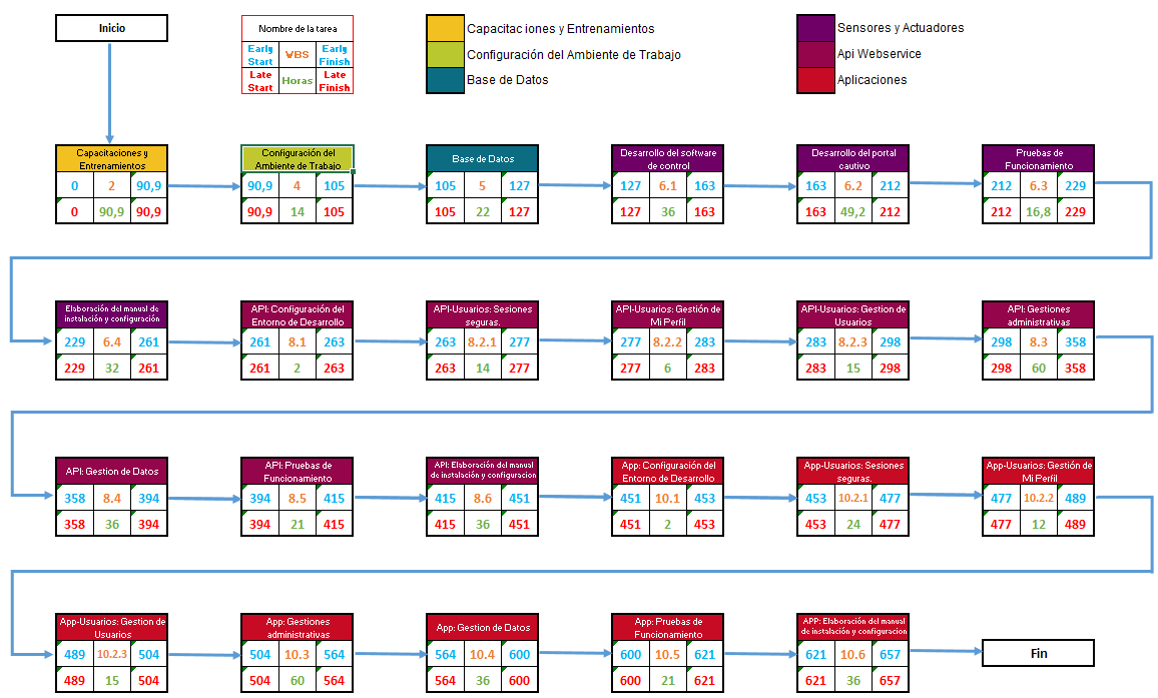
\includegraphics[width=1.4\textwidth]{./Figuras/AoN.png}
\caption{Diagrama en \textit{Activity on Node}}
\label{fig:AoN}
\end{figure}


\end{consigna}

\end{landscape}

\begin{landscape}
%-----------------------------------------------------------
\section{8. Diagrama de Gantt}
\label{sec:gantt}

\begin{consigna}{black}

\vspace{5px}

\begin{figure}[htpb]
	\centering 
	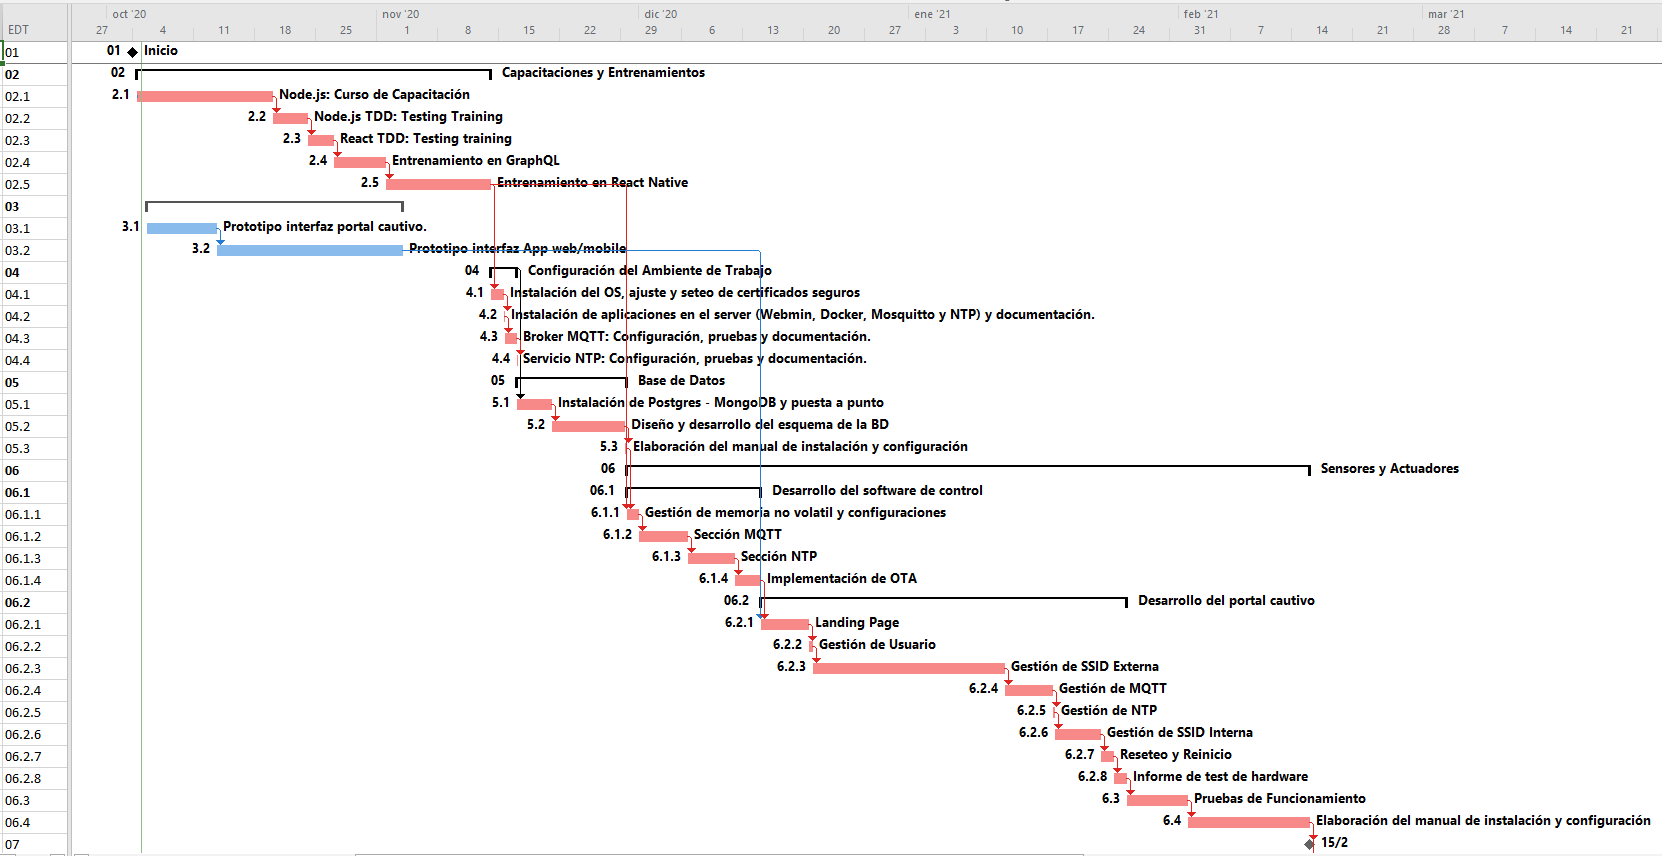
\includegraphics[width=1.4\textwidth]{./Figuras/gantt01.png}
	\caption{Diagrama de Gantt 1 de 3}
	\label{fig:gantt01}
\end{figure}
\vspace{5px}
\newpage
\vspace*{2px}
\begin{figure}[htpb]
	\centering 
	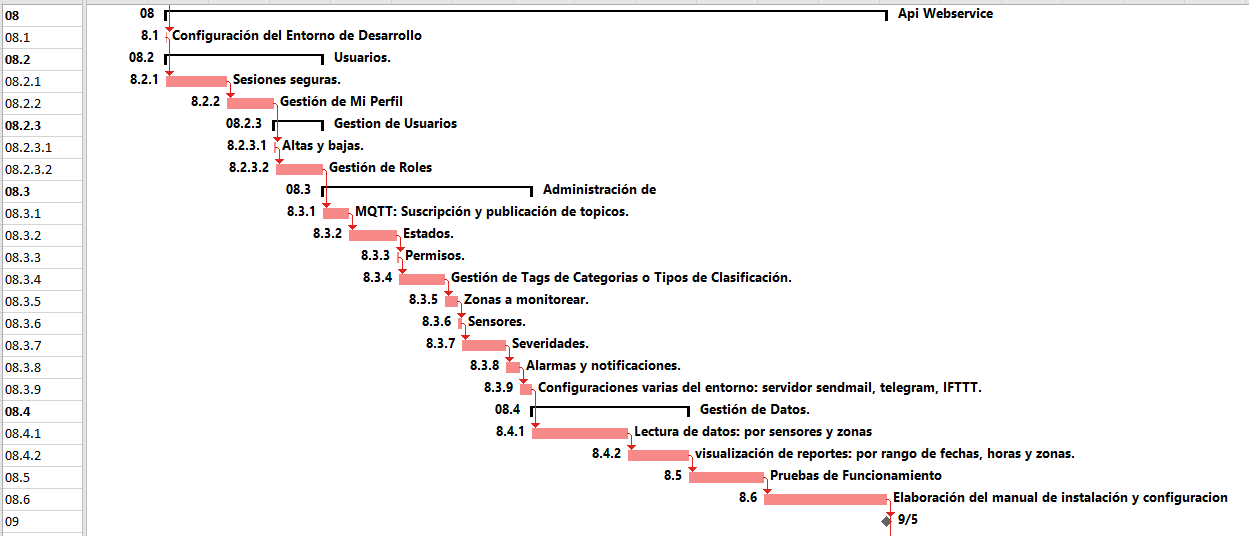
\includegraphics[width=1.3\textwidth]{./Figuras/gantt02.png}
	\caption{Diagrama de Gantt 2 de 3}
	\label{fig:gantt02}
\end{figure}
\vspace{5px}
\newpage
\vspace*{2px}
\begin{figure}[htpb]
	\centering 
	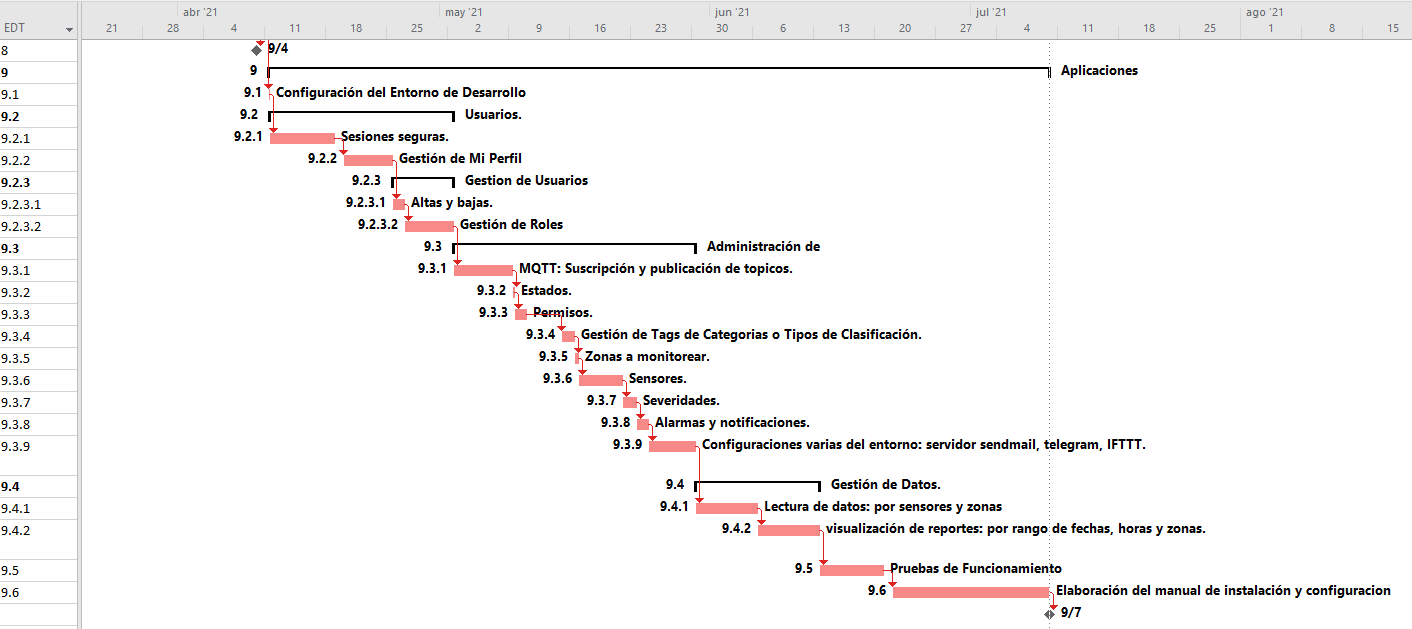
\includegraphics[width=1.4\textwidth]{./Figuras/gantt03.png}
	\caption{Diagrama de Gantt 3 de 3}
	\label{fig:gantt03}
\end{figure}
\vspace{5px}
\newpage

\end{consigna}
\end{landscape}

\begin{landscape}
%-----------------------------------------------------------
\section{9. Matriz de uso de recursos de materiales}
\label{sec:recursos}


\begin{tabularx}{\linewidth}{@{}|p{2cm}|p{11cm}|p{2.4cm}|p{2.4cm}|p{2.4cm}|p{2.4cm}|@{}} %{@{}|c|X|X|X|X|c|@{}}
\hline
\cellcolor[HTML]{C0C0C0} 
	& \cellcolor[HTML]{C0C0C0} 
	& \multicolumn{4}{c}{\cellcolor[HTML]{C0C0C0}Recursos requeridos (horas)} \\ \cline{3-6} 
\multirow{-2}{*}{\cellcolor[HTML]{C0C0C0}\begin{tabular}[c]{@{}c@{}}Código\\ WBS\end{tabular}} & \multirow{-2}{*}{\cellcolor[HTML]{C0C0C0}\begin{tabular}[c]{@{}c@{}}Nombre \\ tarea\end{tabular}} & Developer & PC & Internet & Servidor \\ \hline
1              & \textbf{Inicio}                                                                               & 0    & 0    & 0    & 0    \\
\textbf{2}     & \textbf{Capacitaciones y Entrenamientos}                                                      & 0    & 0    & 0    & 0    \\
2.1            & Entrenamiento en GraphQL                                                                      & 14   & 14   & 14   & 0    \\
2.2            & Entrenamiento en React Native                                                                 & 20   & 20   & 20   & 0    \\
\textbf{3}     & \textbf{Configuración del Ambiente de   Trabajo}                                              & 0    & 0    & 0    & 0    \\
3.1            & Instalación del OS, ajuste y   seteo de certificados seguros                                  & 4    & 4    & 4    & 4    \\
3.2            & Instalación de aplicaciones en   el server (Webmin, Docker, Mosquitto y NTP) y documentación. & 5    & 5    & 5    & 5    \\
3.3            & Broker MQTT: Configuración,   pruebas y documentación.                                        & 3,5  & 3,5  & 3,5  & 3,5  \\
3.4            & Servicio NTP: Configuración,   pruebas y documentación.                                       & 1,5  & 1,5  & 1,5  & 1,5  \\
\textbf{4}     & \textbf{Base de Datos}                                                                        & 0    & 0    & 0    & 0    \\
4.1            & Instalación de Postgres -   MongoDB y puesta a punto                                          & 2    & 2    & 2    & 2    \\
4.2            & Diseño y desarrollo del esquema   de la BD                                                    & 16   & 16   & 16   & 16   \\
4.3            & Elaboración del manual de   instalación y configuración                                       & 4    & 4    & 4    & 4    \\
\textbf{5}     & \textbf{Sensores y Actuadores}                                                                & 0    & 0    & 0    & 0    \\
\textbf{5.1}   & \textbf{Desarrollo del software de   control}                                                 & 0    & 0    & 0    & 0    \\
5.1.1          & Gestión de memoria no volatil y   configuraciones                                             & 6    & 6    & 6    & 6    \\
5.1.2          & Sección MQTT                                                                                  & 12   & 12   & 12   & 12   \\
5.1.3          & Sección NTP                                                                                   & 6    & 6    & 6    & 6    \\
5.1.4          & Implementación de OTA                                                                         & 12   & 12   & 12   & 12   \\
\textbf{5.2}   & \textbf{Desarrollo del portal cautivo}                                                        & 0    & 0    & 0    & 0    \\
5.2.1          & Landing Page                                                                                  & 7,2  & 7,2  & 7,2  & 7,2  \\
5.2.2          & Gestión de Usuario                                                                            & 6    & 6    & 6    & 6    \\
5.2.3          & Gestión de SSID Externa                                                                       & 6    & 6    & 6    & 6    \\
5.2.4          & Gestión de MQTT                                                                               & 6    & 6    & 6    & 6    \\
5.2.5          & Gestión de NTP                                                                                & 6    & 6    & 6    & 6    \\
5.2.6          & Gestión de SSID Interna                                                                       & 6    & 6    & 6    & 6    \\
5.2.7          & Reseteo y Reinicio                                                                            & 6    & 6    & 6    & 6    \\
5.2.8          & Informe de test de hardware                                                                   & 6    & 6    & 6    & 6    \\
5.3            & Pruebas de Funcionamiento                                                                     & 16,8 & 16,8 & 16,8 & 16,8 \\
5.4            & Elaboración del manual de   instalación y configuración                                       & 32   & 32   & 32   & 32   \\
6              & \textbf{Fin de OS Dispositivos}                                                               & 0    & 0    & 0    & 0    \\
\textbf{7}     & \textbf{Api Webservice}                                                                       & 0    & 0    & 0    & 0    \\
7.1            & Configuración del Entorno de   Desarrollo                                                     & 2    & 2    & 2    & 2    \\
\textbf{7.2}   & \textbf{Usuarios.}                                                                            & 0    & 0    & 0    & 0    \\
7.2.1          & Sesiones seguras.                                                                             & 14   & 14   & 14   & 14   \\
7.2.2          & Gestión de Mi Perfil                                                                          & 6    & 6    & 6    & 6    \\
\textbf{7.2.3} & Gestión de Usuarios                                                                           & 0    & 0    & 0    & 0    \\
7.2.3.1        & Altas y bajas.                                                                                & 6    & 6    & 6    & 6    \\
7.2.3.2        & Gestión de Roles                                                                              & 9    & 9    & 9    & 9    \\
\textbf{7.3}   & \textbf{Administración de}                                                                    & 0    & 0    & 0    & 0    \\
7.3.1          & MQTT: Suscripción y publicación   de tópicos.                                                 & 12   & 12   & 12   & 12   \\
7.3.2          & Estados.                                                                                      & 6    & 6    & 6    & 6    \\
7.3.3          & Permisos.                                                                                     & 6    & 6    & 6    & 6    \\
7.3.4          & Gestión de Tags de Categorias o   Tipos de Clasificación.                                     & 6    & 6    & 6    & 6    \\
7.3.5          & Zonas a monitorear.                                                                           & 6    & 6    & 6    & 6    \\
7.3.6          & Sensores.                                                                                     & 6    & 6    & 6    & 6    \\
7.3.7          & Severidades.                                                                                  & 6    & 6    & 6    & 6    \\
7.3.8          & Alarmas y notificaciones.                                                                     & 6    & 6    & 6    & 6    \\
7.3.9          & Configuraciones varias del   entorno: servidor sendmail, telegram, IFTTT.                     & 6    & 6    & 6    & 6    \\
\textbf{7.4}   & \textbf{Gestión de Datos.}                                                                    & 0    & 0    & 0    & 0    \\
7.4.1          & Lectura de datos: por sensores y   zonas                                                      & 18   & 18   & 18   & 18   \\
7.4.2          & visualización de reportes: por   rango de fechas,  y zonas.                                   & 18   & 18   & 18   & 18   \\
7.5            & Pruebas de Funcionamiento                                                                     & 21   & 21   & 21   & 21   \\
7.6            & Elaboración del manual de   instalación y configuración                                       & 36   & 36   & 36   & 36   \\
8              & \textbf{Fin de API}                                                                           & 0    & 0    & 0    & 0    \\
\textbf{9}     & \textbf{Aplicaciones}                                                                         & 0    & 0    & 0    & 0    \\
9.1            & Configuración del Entorno de   Desarrollo                                                     & 2    & 2    & 2    & 2    \\
\textbf{9.2}   & \textbf{Usuarios.}                                                                            & 0    & 0    & 0    & 0    \\
9.2.1          & Sesiones seguras.                                                                             & 24   & 24   & 24   & 24   \\
9.2.2          & Gestión de Mi Perfil                                                                          & 12   & 12   & 12   & 12   \\
\textbf{9.2.3} & \textbf{Gestión de Usuarios}                                                                  & 0    & 0    & 0    & 0    \\
9.2.3.1        & Altas y bajas.                                                                                & 6    & 0    & 0    & 0    \\
9.2.3.2        & Gestión de Roles                                                                              & 9    & 9    & 9    & 9    \\
\textbf{9.3}   & \textbf{Administración de}                                                                    & 0    & 0    & 0    & 0    \\
9.3.1          & MQTT: Suscripción y publicación   de tópicos.                                                 & 12   & 12   & 12   & 12   \\
9.3.2          & Estados.                                                                                      & 6    & 6    & 6    & 6    \\
9.3.3          & Permisos.                                                                                     & 6    & 6    & 6    & 6    \\
9.3.4          & Gestión de Tags de Categorias o   Tipos de Clasificación.                                     & 6    & 6    & 6    & 6    \\
9.3.5          & Zonas a monitorear.                                                                           & 6    & 6    & 6    & 6    \\
9.3.6          & Sensores.                                                                                     & 6    & 6    & 6    & 6    \\
9.3.7          & Severidades.                                                                                  & 6    & 6    & 6    & 6    \\
9.3.8          & Alarmas y notificaciones.                                                                     & 6    & 6    & 6    & 6    \\
9.3.9          & Configuraciones varias del   entorno: servidor sendmail, telegram, IFTTT.                     & 6    & 6    & 6    & 6    \\
\textbf{9.4}   & \textbf{Gestión de Datos.}                                                                    & 0    & 0    & 0    & 0    \\
9.4.1          & Lectura de datos: por sensores y   zonas                                                      & 18   & 18   & 18   & 18   \\
9.4.2          & visualización de reportes: por   rango de fechas,  y zonas.                                   & 18   & 18   & 18   & 18   \\
9.5            & Pruebas de Funcionamiento                                                                     & 21   & 21   & 21   & 21   \\
9.6            & Elaboración del manual de   instalación y configuración                                       & 36   & 36   & 36   & 36   \\
10             & \textbf{Fin del Proyecto}                                                                     &      &      &      &  

\end{tabularx}
\end{landscape}


%-----------------------------------------------------------
\section{10. Presupuesto detallado del proyecto}
\label{sec:presupuesto}

\begin{consigna}{black}
%Si el proyecto es complejo entonces separarlo en partes:
%\begin{itemize}
%\item Un total global, indicando el subtotal acumulado por cada una de las áreas.
%\item El desglose detallado del subtotal de cada una de las áreas.
%\end{itemize}
%
%IMPORTANTE: No olvidarse de considerar los COSTOS INDIRECTOS.

\end{consigna}

%\begin{table}[htpb]
%\centering
\begin{tabularx}{\linewidth}{@{}|X|c|r|r|@{}}
\hline
\rowcolor[HTML]{418ddc} 
\multicolumn{4}{|c|}{\cellcolor[HTML]{418ddc}COSTOS DIRECTOS} \\ \hline
\rowcolor[HTML]{418ddc} 
Descripción & \multicolumn{1}{c|}{\cellcolor[HTML]{418ddc}Cantidad} & \multicolumn{1}{c|}{\cellcolor[HTML]{418ddc}Valor unitario} & \multicolumn{1}{c|}{\cellcolor[HTML]{418ddc}Valor total} \\ \hline
Developer & \multicolumn{1}{c|}{600 horas} & \multicolumn{1}{c|}{379,16/hora} & \multicolumn{1}{c|}{227.496,00} \\ \hline
Internet &\multicolumn{1}{c|}{600 horas} & \multicolumn{1}{c|}{1,11/hora} & \multicolumn{1}{c|}{666,00} \\ \hline 
PC &\multicolumn{1}{c|}{600 horas} & \multicolumn{1}{c|}{3,42/hora} & \multicolumn{1}{c|}{2.052,00} \\ \hline
Servidor &\multicolumn{1}{c|}{566 horas} & \multicolumn{1}{c|}{0,77/hora} & \multicolumn{1}{c|}{435,82} \\ \hline
\multicolumn{3}{|c|}{SUBTOTAL} & \multicolumn{1}{c|}{230.649,82} \\ \hline
\rowcolor[HTML]{418ddc} 

\multicolumn{4}{|c|}{\cellcolor[HTML]{418ddc}COSTOS INDIRECTOS} \\ \hline
\multicolumn{3}{|c|}{30\% de los costos directos.} & \multicolumn{1}{c|}{69.194,95} \\ \hline
\multicolumn{3}{|c|}{SUBTOTAL} & \multicolumn{1}{c|}{69.194,95} \\ \hline

\rowcolor[HTML]{aad80e}
\multicolumn{3}{|c|}{TOTAL} & 299.844,77
   \\ \hline
\end{tabularx}


\begin{landscape}
%\end{table}


%-----------------------------------------------------------
\section{11. Matriz de asignación de responsabilidades}
\label{sec:responsabilidades}
\begin{consigna}{black}
%Establecer la matriz de asignación de responsabilidades y el manejo de la autoridad completando la siguiente tabla:

%\begin{table}[htpb]
%\centering
%\resizebox{\textwidth}{!}{%
\begin{tabularx}{\linewidth}{@{}|p{1.3cm}|p{9.3cm}|p{3cm}|p{3cm}|p{3cm}|p{3cm}|@{}}%{|c|c|c|c|c|c|}
\hline
\rowcolor[HTML]{418ddc} \cellcolor[HTML]{418ddc} & \cellcolor[HTML]{418ddc} & \multicolumn{4}{c|}{\cellcolor[HTML]{418ddc}Listar todos los nombres y roles del proyecto} \\ \cline{3-6} 
\rowcolor[HTML]{418ddc} \cellcolor[HTML]{418ddc} & \cellcolor[HTML]{418ddc} &  Responsable & Orientador & Equipo & Cliente \\ \cline{3-6} 
\rowcolor[HTML]{418ddc} \multirow{-3}{*}{\cellcolor[HTML]{418ddc}\begin{tabular}[c]{@{}c@{}}Código\\ WBS\end{tabular}} &
\multirow{-3}{*}{\cellcolor[HTML]{418ddc}Nombre de la tarea} & \authorname & \supname &  --- & \clientename \\ \hline
1 & \textbf{Inicio}                                                                               				       & \textbf{-} & \textbf{-} & \textbf{-} & \textbf{-} \\
2                      & \textbf{Capacitaciones y Entrenamientos}                                                      & \textbf{P} & \textbf{I} & \textbf{-} & \textbf{I} \\
2.1                    & Entrenamiento en GraphQL                                                                      & P          & \textbf{-} & \textbf{-} & \textbf{-} \\
2.2                    & Entrenamiento en React Native                                                                 & P          & \textbf{-} & \textbf{-} & \textbf{-} \\
3                      & \textbf{Configuración del Ambiente de   Trabajo}                                              & \textbf{P} & \textbf{C} & \textbf{-} & \textbf{I} \\
3.1                    & Instalación del OS, ajuste y   seteo de certificados seguros                                  & P          & \textbf{-} & \textbf{-} & \textbf{-} \\
3.2                    & Instalación de aplicaciones en   el server (Webmin, Docker, Mosquitto y NTP) y documentación. & P          & \textbf{-} & \textbf{-} & \textbf{-} \\
3.3                    & Broker MQTT: Configuración,   pruebas y documentación.                                        & P          & \textbf{-} & \textbf{-} & \textbf{-} \\
3.4                    & Servicio NTP: Configuración,   pruebas y documentación.                                       & P          & \textbf{-} & \textbf{-} & \textbf{-} \\
4                      & \textbf{Base de Datos}                                                                        & \textbf{P} & \textbf{A} & \textbf{-} & \textbf{I} \\
4.1                    & Instalación de Postgres -   MongoDB y puesta a punto                                          & P          & \textbf{-} & \textbf{-} & \textbf{-} \\
4.2                    & Diseño y desarrollo del esquema   de la BD                                                    & P          & \textbf{-} & \textbf{-} & \textbf{-} \\
4.3                    & Elaboración del manual de   instalación y configuración                                       & P          & \textbf{-} & \textbf{-} & \textbf{-} \\
5                      & \textbf{Sensores y Actuadores}                                                                & \textbf{P} & \textbf{A} & \textbf{-} & \textbf{I} \\
5.1                    & \textbf{Desarrollo del software de   control}                                                 & P          & C          & -          & I          \\
5.1.1                  & Gestión de memoria no volátil y   configuraciones                                             & P          & \textbf{-} & \textbf{-} & \textbf{-} \\
5.1.2                  & Sección MQTT                                                                                  & P          & \textbf{-} & \textbf{-} & \textbf{-} \\
5.1.3                  & Sección NTP                                                                                   & P          & \textbf{-} & \textbf{-} & \textbf{-} \\
5.1.4                  & Implementación de OTA                                                                         & P          & \textbf{-} & \textbf{-} & \textbf{-} \\
5.2                    & \textbf{Desarrollo del portal cautivo}                                                        & P          & C          & -          & I          \\
5.2.1                  & Landing Page                                                                                  & P          & \textbf{-} & \textbf{-} & \textbf{-} \\
5.2.2                  & Gestión de Usuario                                                                            & P          & \textbf{-} & \textbf{-} & \textbf{-} \\
5.2.3                  & Gestión de SSID Externa                                                                       & P          & \textbf{-} & \textbf{-} & \textbf{-} \\
5.2.4                  & Gestión de MQTT                                                                               & P          & \textbf{-} & \textbf{-} & \textbf{-} \\
5.2.5                  & Gestión de NTP                                                                                & P          & \textbf{-} & \textbf{-} & \textbf{-} \\
5.2.6                  & Gestión de SSID Interna                                                                       & P          & \textbf{-} & \textbf{-} & \textbf{-} \\
5.2.7                  & Reseteo y Reinicio                                                                            & P          & \textbf{-} & \textbf{-} & \textbf{-} \\
5.2.8                  & Informe de test de hardware                                                                   & P          & \textbf{-} & \textbf{-} & \textbf{-} \\
5.3                    & Pruebas de Funcionamiento                                                                     & P          & C          & -          & I          \\
5.4                    & Elaboración del manual de   instalación y configuración                                       & P          & C          & -          & C          \\
6                      & \textbf{Fin de OS Dispositivos}                                                               & \textbf{-} & \textbf{-} & \textbf{-} & \textbf{-} \\
7                      & \textbf{Api Webservice}                                                                       & \textbf{P} & \textbf{A} & \textbf{-} & \textbf{I} \\
7.1                    & Configuración del Entorno de   Desarrollo                                                     & P          & \textbf{-} & \textbf{-} & \textbf{-} \\
7.2                    & \textbf{Usuarios.}                                                                            & \textbf{P} & \textbf{A} & \textbf{-} & \textbf{I} \\
7.2.1                  & Sesiones seguras.                                                                             & P          & \textbf{-} & \textbf{-} & \textbf{-} \\
7.2.2                  & Gestión de Mi Perfil                                                                          & P          & \textbf{-} & \textbf{-} & \textbf{-} \\
7.2.3                  & \textbf{Gestión de Usuarios}                                                                  & \textbf{P} & \textbf{A} & \textbf{-} & \textbf{I} \\
7.2.3.1                & Altas y bajas.                                                                                & P          & \textbf{-} & \textbf{-} & \textbf{-} \\
7.2.3.2                & Gestión de Roles                                                                              & P          & \textbf{-} & \textbf{-} & \textbf{-} \\
7.3                    & \textbf{Administración de}                                                                    & \textbf{P} & \textbf{A} & \textbf{-} & \textbf{I} \\
7.3.1                  & MQTT: Suscripción y publicación   de tópicos.                                                 & P          & \textbf{-} & \textbf{-} & \textbf{-} \\
7.3.2                  & Estados.                                                                                      & P          & \textbf{-} & \textbf{-} & \textbf{-} \\
7.3.3                  & Permisos.                                                                                     & P          & \textbf{-} & \textbf{-} & \textbf{-} \\
7.3.4                  & Gestión de Tags de Categorias o   Tipos de Clasificación.                                     & P          & \textbf{-} & \textbf{-} & \textbf{-} \\
7.3.5                  & Zonas a monitorear.                                                                           & P          & \textbf{-} & \textbf{-} & \textbf{-} \\
7.3.6                  & Sensores.                                                                                     & P          & \textbf{-} & \textbf{-} & \textbf{-} \\
7.3.7                  & Severidades.                                                                                  & P          & \textbf{-} & \textbf{-} & \textbf{-} \\
7.3.8                  & Alarmas y notificaciones.                                                                     & P          & \textbf{-} & \textbf{-} & \textbf{-} \\
7.3.9                  & Configuraciones varias del   entorno: servidor sendmail, telegram, IFTTT.                     & P          & \textbf{-} & \textbf{-} & \textbf{-} \\
7.4                    & \textbf{Gestión de Datos.}                                                                    & \textbf{P} & \textbf{A} & \textbf{-} & \textbf{I} \\
7.4.1                  & Lectura de datos: por sensores y   zonas                                                      & P          & \textbf{-} & \textbf{-} & \textbf{-} \\
7.4.2                  & visualización de reportes: por   rango de fechas,  y zonas.                                   & P          & \textbf{-} & \textbf{-} & \textbf{-} \\
7.5                    & Pruebas de Funcionamiento                                                                     & \textbf{P} & \textbf{C} & \textbf{-} & \textbf{-} \\
7.6                    & Elaboración del manual de   instalación y configuración                                       & \textbf{P} & \textbf{A} & \textbf{-} & \textbf{I} \\
8                      & \textbf{Fin de API}                                                                           &            & \textbf{-} & \textbf{-} & \textbf{-} \\
9                      & \textbf{Aplicaciones}                                                                         & \textbf{P} & \textbf{A} & \textbf{-} & \textbf{I} \\
9.1                    & Configuración del Entorno de   Desarrollo                                                     & P          & \textbf{-} & \textbf{-} & \textbf{-} \\
9.2                    & \textbf{Usuarios.}                                                                            & \textbf{P} & \textbf{A} & \textbf{-} & \textbf{I} \\
9.2.1                  & Sesiones seguras.                                                                             & P          & \textbf{-} & \textbf{-} & \textbf{-} \\
9.2.2                  & Gestión de Mi Perfil                                                                          & P          & \textbf{-} & \textbf{-} & \textbf{-} \\
9.2.3                  & \textbf{Gestión de Usuarios}                                                                  & \textbf{P} & \textbf{A} & \textbf{-} & \textbf{I} \\
9.2.3.1                & Altas y bajas.                                                                                & P          & \textbf{-} & \textbf{-} & \textbf{-} \\
9.2.3.2                & Gestión de Roles                                                                              & P          & \textbf{-} & \textbf{-} & \textbf{-} \\
9.3                    & \textbf{Administración de}                                                                    & \textbf{P} & \textbf{A} & \textbf{-} & \textbf{I} \\
9.3.1                  & MQTT: Suscripción y publicación   de tópicos.                                                 & P          & \textbf{-} & \textbf{-} & \textbf{-} \\
9.3.2                  & Estados.                                                                                      & P          & \textbf{-} & \textbf{-} & \textbf{-} \\
9.3.3                  & Permisos.                                                                                     & P          & \textbf{-} & \textbf{-} & \textbf{-} \\
9.3.4                  & Gestión de Tags de Categorias o   Tipos de Clasificación.                                     & P          & \textbf{-} & \textbf{-} & \textbf{-} \\
9.3.5                  & Zonas a monitorear.                                                                           & P          & \textbf{-} & \textbf{-} & \textbf{-} \\
9.3.6                  & Sensores.                                                                                     & P          & \textbf{-} & \textbf{-} & \textbf{-} \\
9.3.7                  & Severidades.                                                                                  & P          & \textbf{-} & \textbf{-} & \textbf{-} \\
9.3.8                  & Alarmas y notificaciones.                                                                     & P          & \textbf{-} & \textbf{-} & \textbf{-} \\
9.3.9                  & Configuraciones varias del   entorno: servidor sendmail, telegram, IFTTT.                     & P          & \textbf{-} & \textbf{-} & \textbf{-} \\
9.4                    & \textbf{Gestión de Datos.}                                                                    & \textbf{P} & \textbf{A} & \textbf{-} & \textbf{I} \\
9.4.1                  & Lectura de datos: por sensores y   zonas                                                      & P          & \textbf{-} & \textbf{-} & \textbf{-} \\
9.4.2                  & visualización de reportes: por   rango de fechas,  y zonas.                                   & P          & \textbf{-} & \textbf{-} & \textbf{-} \\
9.5                    & Pruebas de Funcionamiento                                                                     & \textbf{P} & \textbf{C} & \textbf{-} & \textbf{-} \\
9.6                    & Elaboración del manual de   instalación y configuración                                       & \textbf{P} & \textbf{C} & \textbf{-} & \textbf{C} \\
10                     & \textbf{Fin del Proyecto}                                                                     & \textbf{-} & \textbf{-} & \textbf{-} & \textbf{-}
\end{tabularx}

{\footnotesize
Referencias:
\begin{itemize}
	\item P = Responsabilidad Primaria
	\item S = Responsabilidad Secundaria
	\item A = Aprobación
	\item I = Informado
	\item C = Consultado
\end{itemize}
} %footnotesize

%Una de las columnas debe ser para el Director, ya que se supone que participará en el proyecto.
%A su vez se debe cuidar que no queden muchas tareas seguidas sin ``A'' o ``I''.
%
%Importante: es redundante poner ``I/A'' o ``I/C'', porque para aprobarlo o responder consultas primero la persona debe ser informada.

\end{consigna}
\end{landscape}

%-----------------------------------------------------------
\section{12. Gestión de riesgos}
\label{sec:riesgos}

\begin{consigna}{black}
a) Identificación de los riesgos:

Riesgo 1: Falta de tiempo para adquirir los conocimientos necesarios para desarrollar y culminar todo el proyecto.
\begin{itemize}
\item Severidad (S): 7, Puede impactar en la calidad del software y por ende en el desarrollo de los requerimientos.
\item Ocurrencia (O): 2, Por experiencia previa se sabe que dicho riesgo se mitiga con capacitaciones y entrenamientos.
\end{itemize}
		
Riesgo 2: Mala estimación de la planificación. Incumplimiento de fecha pautada.
\begin{itemize}
\item Severidad (S): 9, Riesgo alto dado que se requiere la culminación de todo el proyecto.
\item Ocurrencia (O): 4, Se cuenta con una experiencia en planificación de sólo 1 año.
\end{itemize}
		
Riesgo 3: La estación de trabajo del desarrollador del proyecto sufre daños irreversibles.  
\begin{itemize}
\item Severidad (S): 10, El desarrollador cuenta con un equipo personal a dedicación exclusiva para el proyecto.
\item Ocurrencia (O): 2, Es baja dado que el equipo es relativamente nuevo y cuenta con mantenimientos periódicos.
\end{itemize}

Riesgo 4: Que lleguen a existir requerimientos no contemplados en el levantamiento inicial.  
\begin{itemize}
\item Severidad (S): 6, A medida que el proyecto se vaya desarrollando es posible que aparezcan requerimientos importantes no contemplados inicialmente ya sea por casos detectados por desarrollo o el cliente.
\item Ocurrencia (O): 3, Es posible que hayan quedado algunos requerimientos funcionales sin levantar de los cuales su desarrollo queda supeditado a la relevancia.
\end{itemize}		

Riesgo 5: Pérdida o daño de los archivos fuentes de los componentes del proyecto. 
\begin{itemize}
\item Severidad (S): 9, Implica perdida de trabajo y retraso en el desarrollo con la consecuente prolongación de la fecha de finalización.
\item Ocurrencia (O): 1, Durante el desarrollo del proyecto se utilizará un sistema de control de versiones, backup en NAS local y en Cloud.
\end{itemize}	
							
\newpage		
b) Tabla de gestión de riesgos: 

\begin{table}[htpb]
\centering
\begin{tabularx}{\linewidth}{@{}|X|c|c|c|c|c|c|@{}}
\hline
\rowcolor[HTML]{418ddc} 
Riesgo & S & O & RPN & S* & O* & RPN* \\ \hline
Riesgo 1 & 7  & 2 & 14 &   &   &    \\
Riesgo 2 & 9  & 4 & 36 & 5 & 2 & 10 \\
Riesgo 3 & 10 & 2 & 20 & 3 & 1 &    \\
Riesgo 4 & 6  & 3 & 18 &   &   &    \\
Riesgo 5 & 9  & 1 & 9  &   &   &
\end{tabularx}
\end{table}

Criterio adoptado: 
Se tomarán medidas de mitigación en los riesgos cuyos números de RPN sean mayores o iguales a 20.
							
c) Plan de mitigación de los riesgos que originalmente excedían el RPN máximo establecido:		
					
Riesgo 2: Mala estimación de la planificación. Incumplimiento de fecha pautada.
\begin{itemize}
\item Plan de mitigación: Contar con la asesoría de expertos en el tema para hacer una mejor estimación.
\item Severidad (S): 5, Se cuenta con el apoyo de un Scrum Master para verificar las estimaciones.
\item Ocurrencia (O): 2, Es un colega del trabajo que está disponible a requerimiento del desarrollador previa agenda.
\end{itemize}

Riesgo 3: La estación de trabajo del desarrollador del proyecto sufre daños irreversibles.  
\begin{itemize}
\item Plan de mitigación: Contar con un equipo de respaldo para seguir desarrollando.
\item Severidad (S): 3, Se puede contar con el equipo asignado por razones de trabajo.
\item Ocurrencia (O): 1, El equipo se encuentra a disposición del desarrollador.
\end{itemize}

\end{consigna}


%-----------------------------------------------------------
\section{13. Gestión de la calidad}
\label{sec:calidad}

\begin{consigna}{black}
%Para cada uno de los requerimientos del proyecto indique:
%\begin{itemize} 
%\item Req \#1: copiar acá el requerimiento.
%
%Verificación y validación:
%
%\begin{itemize}
%\item Verificación para confirmar si se cumplió con lo requerido antes de mostrar el sistema al cliente. Detallar 
%\item Validación con el cliente para confirmar que está de acuerdo en que se cumplió con lo requerido. Detallar  
%\end{itemize}
%
%\end{itemize}
%
%Tener en cuenta que en este contexto se pueden mencionar simulaciones, cálculos, revisión de hojas de datos, consulta con expertos, mediciones, etc.
\begin{itemize}
\item Req.1 Grupo de requerimientos asociados con sensores y actuadores: 
	\begin{description}
		\item Verificación: Pruebas unitarias y de integración sobre las funciones descritas.
		\item Validación: Pruebas sobre el producto final.
	\end{description}	
\item Req.2 Grupo de requerimientos asociados con el servicio NTP:
		\begin{description}
			\item Verificación: Pruebas unitarias y de integración sobre las funciones descritas.
			\item Validación: Pruebas sobre el producto final.
		\end{description}
\item Req.3 Grupo de requerimientos asociados con la base de datos:
		\begin{description}
			\item Verificación: Pruebas unitarias y de integración sobre las funciones descritas.
			\item Validación: Pruebas sobre el producto final.
		\end{description}	
\item Req.4 Grupo de requerimientos asociados con el broker MQTT:
		\begin{description}
			\item Verificación: Pruebas unitarias y de integración sobre las funciones descritas.
			\item Validación: Pruebas sobre el producto final.
		\end{description}	
\item Req.5 Grupo de requerimientos asociados con Api - WebService:
		\begin{description}
			\item Verificación: Pruebas unitarias y de integración sobre las funciones descritas.
			\item Validación: Pruebas sobre el producto final.
		\end{description}			
\item Req.6 Grupo de requerimientos asociados con la App:
		\begin{description}
			\item Verificación: Pruebas unitarias y de integración sobre las funciones descritas.
			\item Validación: Pruebas sobre el producto final.
		\end{description}	
\end{itemize}

\end{consigna}


\begin{landscape}
%\newpage
%-----------------------------------------------------------
\section{14. Comunicación del proyecto}
\label{sec:comunicaciones}

El plan de comunicación del proyecto es el siguiente:

%\begin{table}[htpb]
%\begin{tabularx}{\linewidth}{@{}|X{1.3cm}|p{17cm}|p{1.7cm}|p{1.5cm}|p{1.7cm}|@{}}
\begin{tabularx}{\linewidth}{@{}|p{6.8cm}|p{4cm}|p{4cm}|p{4cm}|p{2cm}|p{2cm}|@{}}
\hline
\rowcolor[HTML]{418ddc} 
\multicolumn{6}{|c|}{\cellcolor[HTML]{418ddc}PLAN DE COMUNICACIÓN DEL PROYECTO}           \\ \hline
\rowcolor[HTML]{418ddc} 
¿Qué   comunicar?                                                 & Audiencia             & Propósito                                                & Frecuencia                     & Método de comunicac. & Responsable       \\
Plan de   Proyecto                                                & Todos los interesados & Actualización de información                             & Inicio del proyecto            & Email                & Katherine Aguirre \\
Avance   en el desarrollo del software para sensores y actuadores & Todos los interesados & Actualización de información                             & Mensual                        & Email                & Katherine Aguirre \\
Avance   en el desarrollo de la API                               & Todos los interesados & Actualización de información                             & Mensual                        & Email                & Katherine Aguirre \\
Avance   en el desarrollo de la Aplicación                        & Todos los interesados & Actualización de información                             & Mensual                        & Email                & Katherine Aguirre \\
Estado   de avance general del proyecto                           & Todos los interesados & Actualización de información                             & A requerimiento del interesado & Email                & Katherine Aguirre \\
Grado de   avance                                                 & Todos los interesados & Actualización de información                             & Cada release                   & Email                & Katherine Aguirre \\
Desviaciones   del plan de trabajo                                & Todos los interesados & Advertir retrasos o   inconvenientes y buscar soluciones & Cuando sucedan                 & Email                & Katherine Aguirre \\
Fin del   proyecto                                                & Todos los interesados & Informar                                                 & Fin del proyecto               & Email                & Katherine Aguirre
\\ \hline
\end{tabularx}
%\end{table}


%-----------------------------------------------------------
\section{15. Gestión de compras}
\label{sec:compras}

\begin{consigna}{black}
La gestión de compras la realiza el responsable del Proyecto.
a) Para el caso de compra de hardware, se seleccionarán proveedores nacionales que cuenten con stock de los componentes requeridos y presenten una cotización de menor valor de los mismos. 
b) Como los componentes a utilizar pueden ser adquiridos con varios proveedores se descarta el análisis de éstos.
\end{consigna}
\end{landscape}
\begin{landscape}
%-----------------------------------------------------------
\section{16. Seguimiento y control}
\label{sec:seguimiento}

\begin{consigna}{black}
%Para cada tarea del proyecto establecer la frecuencia y los indicadores con los se seguirá su avance y quién será el responsable de hacer dicho seguimiento y a quién debe comunicarse la situación (en concordancia con el Plan de Comunicación del proyecto).
%
%El indicador de avance tiene que ser algo medible, mejor incluso si se puede medir en \% de avance. Por ejemplo,se pueden indicar en esta columna cosas como ``cantidad de conexiones ruteadeas'' o ``cantidad de funciones implementadas'', pero no algo genérico y ambiguo como ``\%'', porque el lector no sabe porcentaje de qué cosa.

\end{consigna}

%\begin{longtable}{|m{1cm}|m{3.5cm}|m{2.2cm}|m{2cm}|m{3cm}|m{1.5cm}|}
%\hline
%\rowcolor[HTML]{418ddc} 
%\multicolumn{6}{|c|}{\cellcolor[HTML]{418ddc}SEGUIMIENTO DE AVANCE}                                                                       \\ \hline
%\rowcolor[HTML]{418ddc} 
%Tarea del WBS 			& Indicador de avance & Frecuencia de reporte & Resp. de seguimiento & Persona a ser informada & Método de comunic. \\ \hline
%\endfirsthead
%
%\hline
%\rowcolor[HTML]{418ddc} 
%\multicolumn{6}{c}{\cellcolor[HTML]{418ddc}SEGUIMIENTO DE AVANCE}                                                                       \\ \hline
%\rowcolor[HTML]{418ddc} 
%Tarea del WBS 			& Indicador de avance & Frecuencia de reporte & Resp. de seguimiento & Persona a ser informada & Método de comunic. \\ \hline
%\endhead
%
%\multicolumn{6}{c}{Continúa}
%\endfoot
%
%\endlastfoot
%
%1	& Fecha de inicio  & Única vez al comienzo & \authorname & \clientename, \supname & email \\ \hline
%2.1	& Avance de las subtareas  & Mensual mientras dure la tarea & \authorname & \clientename, \supname & email \\ \hline
%
%\end{longtable}

%\begin{table}[!htpb]
%\centering
%\begin{tabularx}{\linewidth}{@{}|X|X|X|X|X|X|@{}}
\begin{tabularx}{\linewidth}{@{}|X|C{8cm}|C{4cm}|C{2cm}|C{4cm}|C{2cm}|@{}}
\hline
\rowcolor[HTML]{418ddc} 
\multicolumn{6}{|c|}{\cellcolor[HTML]{418ddc}SEGUIMIENTO DE AVANCE}                                                                       \\ \hline
\rowcolor[HTML]{418ddc} 
Tarea del WBS & Indicador de avance & Frecuencia de reporte & Resp. de seguimiento & Persona a ser informada & Método de comunic. \\ \hline
1             & Fecha   de inicio                                                                                            & Única vez al comienzo            & \authorname & \clientename,   \supname & Email \\
2, 3, 4       & Capacitaciones y configuraciones.                                                                            & Mensual   mientras dure la tarea & \authorname & \clientename,   \supname & Email \\
5.1           & \%   de avance en el desarrollo del software de control del sensor.                                           & Mensual   mientras dure la tarea & \authorname & \clientename,   \supname & Email \\
5.2, 5.3, 5.4 & \% de avance en el Desarrollo del portal cautivo del   sensor, resultado de pruebas y documentación generada. & Mensual   mientras dure la tarea & \authorname & \clientename,   \supname & Email \\
7.2           & \% de avance en la Api Usuarios.                                                                              & Mensual   mientras dure la tarea & \authorname & \clientename,   \supname & Email \\
7.3           & \% de avance en la Api Administración                                                                         & Mensual   mientras dure la tarea & \authorname & \clientename,   \supname & Email \\
7.4, 7.5, 7.6 & \% de avance en la Api Gestión de Datos, resultado de   pruebas y documentación generada.                     & Mensual   mientras dure la tarea & \authorname & \clientename,   \supname & Email \\
9.2           & \% de avance en la App sección de Usuarios.                                                                   & Mensual   mientras dure la tarea & \authorname & \clientename,   \supname & Email \\
9.3           & \% de avance en la App sección de Administración                                                               & Mensual   mientras dure la tarea & \authorname & \clientename,   \supname & Email \\
9.4, 9.5, 9.6 & \% de avance en la App sección de Gestión de Datos,   resultado de las pruebas y documentación generada.      & Mensual   mientras dure la tarea & \authorname & \clientename,   \supname & Email \\
9.6           & Fin del Proyecto                                                                                             & Única vez al final               & \authorname & \clientename,   \supname & Email
\end{tabularx}%
%}
%\end{table}
\end{landscape}

%-----------------------------------------------------------
\section{17. Procesos de cierre}    
\label{sec:cierre}

\begin{consigna}{black}
\begin{itemize}
\item Pautas de trabajo que se seguirán para analizar si se respetó el Plan de Proyecto original:
	\begin{description}
		\item Encargada: \authorname
		\item Al concluir el proyecto se realizará una reunión virtual con los interesados del proyecto para evaluar el plan ejecutado en comparación con el planificado.
		\item Serán analizados los requerimientos iniciales y el grado de ajuste a lo planteado de los mismos
	\end{description}
\item Identificación de las técnicas y procedimientos útiles e inútiles que se utilizaron, y los problemas que surgieron y cómo se solucionaron:
	\begin{description}
		\item Encargada: \authorname
		\item Se realizará un paper a modo de presentación donde se expondrá la información relacionada a los tiempos en relación al plan y al real, causas y correcciones de las desviaciones o pronta finalización.
		\item Igualmente se incorporará una tabla donde se tabule que se hizo bien y se mantendría, que se pudo haber mejorado y que fue mal.
	\end{description}
\item Indicar quién organizará el acto de agradecimiento a todos los interesados, y en especial al equipo de trabajo y colaboradores:
	\begin{description}
		\item Encargada: \authorname
		\item Serán invitados los colaboradores a la exposición final del proyecto. 
		\item Así mismo será realizada una mención pública y agradecimiento de los colaboradores el la memoria final del proyecto
	\end{description}
\end{itemize}

\end{consigna}


\end{document}
